% Options for packages loaded elsewhere
% Options for packages loaded elsewhere
\PassOptionsToPackage{unicode}{hyperref}
\PassOptionsToPackage{hyphens}{url}
\PassOptionsToPackage{dvipsnames,svgnames,x11names}{xcolor}
%
\documentclass[
  11pt,
]{article}
\usepackage{xcolor}
\usepackage[margin=2.5cm]{geometry}
\usepackage{amsmath,amssymb}
\setcounter{secnumdepth}{5}
\usepackage{iftex}
\ifPDFTeX
  \usepackage[T1]{fontenc}
  \usepackage[utf8]{inputenc}
  \usepackage{textcomp} % provide euro and other symbols
\else % if luatex or xetex
  \usepackage{unicode-math} % this also loads fontspec
  \defaultfontfeatures{Scale=MatchLowercase}
  \defaultfontfeatures[\rmfamily]{Ligatures=TeX,Scale=1}
\fi
\usepackage{lmodern}
\ifPDFTeX\else
  % xetex/luatex font selection
\fi
% Use upquote if available, for straight quotes in verbatim environments
\IfFileExists{upquote.sty}{\usepackage{upquote}}{}
\IfFileExists{microtype.sty}{% use microtype if available
  \usepackage[]{microtype}
  \UseMicrotypeSet[protrusion]{basicmath} % disable protrusion for tt fonts
}{}
\makeatletter
\@ifundefined{KOMAClassName}{% if non-KOMA class
  \IfFileExists{parskip.sty}{%
    \usepackage{parskip}
  }{% else
    \setlength{\parindent}{0pt}
    \setlength{\parskip}{6pt plus 2pt minus 1pt}}
}{% if KOMA class
  \KOMAoptions{parskip=half}}
\makeatother
% Make \paragraph and \subparagraph free-standing
\makeatletter
\ifx\paragraph\undefined\else
  \let\oldparagraph\paragraph
  \renewcommand{\paragraph}{
    \@ifstar
      \xxxParagraphStar
      \xxxParagraphNoStar
  }
  \newcommand{\xxxParagraphStar}[1]{\oldparagraph*{#1}\mbox{}}
  \newcommand{\xxxParagraphNoStar}[1]{\oldparagraph{#1}\mbox{}}
\fi
\ifx\subparagraph\undefined\else
  \let\oldsubparagraph\subparagraph
  \renewcommand{\subparagraph}{
    \@ifstar
      \xxxSubParagraphStar
      \xxxSubParagraphNoStar
  }
  \newcommand{\xxxSubParagraphStar}[1]{\oldsubparagraph*{#1}\mbox{}}
  \newcommand{\xxxSubParagraphNoStar}[1]{\oldsubparagraph{#1}\mbox{}}
\fi
\makeatother


\usepackage{longtable,booktabs,array}
\usepackage{calc} % for calculating minipage widths
% Correct order of tables after \paragraph or \subparagraph
\usepackage{etoolbox}
\makeatletter
\patchcmd\longtable{\par}{\if@noskipsec\mbox{}\fi\par}{}{}
\makeatother
% Allow footnotes in longtable head/foot
\IfFileExists{footnotehyper.sty}{\usepackage{footnotehyper}}{\usepackage{footnote}}
\makesavenoteenv{longtable}
\usepackage{graphicx}
\makeatletter
\newsavebox\pandoc@box
\newcommand*\pandocbounded[1]{% scales image to fit in text height/width
  \sbox\pandoc@box{#1}%
  \Gscale@div\@tempa{\textheight}{\dimexpr\ht\pandoc@box+\dp\pandoc@box\relax}%
  \Gscale@div\@tempb{\linewidth}{\wd\pandoc@box}%
  \ifdim\@tempb\p@<\@tempa\p@\let\@tempa\@tempb\fi% select the smaller of both
  \ifdim\@tempa\p@<\p@\scalebox{\@tempa}{\usebox\pandoc@box}%
  \else\usebox{\pandoc@box}%
  \fi%
}
% Set default figure placement to htbp
\def\fps@figure{htbp}
\makeatother


% definitions for citeproc citations
\NewDocumentCommand\citeproctext{}{}
\NewDocumentCommand\citeproc{mm}{%
  \begingroup\def\citeproctext{#2}\cite{#1}\endgroup}
\makeatletter
 % allow citations to break across lines
 \let\@cite@ofmt\@firstofone
 % avoid brackets around text for \cite:
 \def\@biblabel#1{}
 \def\@cite#1#2{{#1\if@tempswa , #2\fi}}
\makeatother
\newlength{\cslhangindent}
\setlength{\cslhangindent}{1.5em}
\newlength{\csllabelwidth}
\setlength{\csllabelwidth}{3em}
\newenvironment{CSLReferences}[2] % #1 hanging-indent, #2 entry-spacing
 {\begin{list}{}{%
  \setlength{\itemindent}{0pt}
  \setlength{\leftmargin}{0pt}
  \setlength{\parsep}{0pt}
  % turn on hanging indent if param 1 is 1
  \ifodd #1
   \setlength{\leftmargin}{\cslhangindent}
   \setlength{\itemindent}{-1\cslhangindent}
  \fi
  % set entry spacing
  \setlength{\itemsep}{#2\baselineskip}}}
 {\end{list}}
\usepackage{calc}
\newcommand{\CSLBlock}[1]{\hfill\break\parbox[t]{\linewidth}{\strut\ignorespaces#1\strut}}
\newcommand{\CSLLeftMargin}[1]{\parbox[t]{\csllabelwidth}{\strut#1\strut}}
\newcommand{\CSLRightInline}[1]{\parbox[t]{\linewidth - \csllabelwidth}{\strut#1\strut}}
\newcommand{\CSLIndent}[1]{\hspace{\cslhangindent}#1}



\setlength{\emergencystretch}{3em} % prevent overfull lines

\providecommand{\tightlist}{%
  \setlength{\itemsep}{0pt}\setlength{\parskip}{0pt}}



 


\usepackage{booktabs}
\usepackage{longtable}
\usepackage{array}
\usepackage{multirow}
\usepackage{wrapfig}
\usepackage{float}
\usepackage{colortbl}
\usepackage{pdflscape}
\usepackage{tabu}
\usepackage{threeparttable}
\usepackage{threeparttablex}
\usepackage[normalem]{ulem}
\usepackage{makecell}
\usepackage{xcolor}
\makeatletter
\@ifpackageloaded{caption}{}{\usepackage{caption}}
\AtBeginDocument{%
\ifdefined\contentsname
  \renewcommand*\contentsname{Table of contents}
\else
  \newcommand\contentsname{Table of contents}
\fi
\ifdefined\listfigurename
  \renewcommand*\listfigurename{List of Figures}
\else
  \newcommand\listfigurename{List of Figures}
\fi
\ifdefined\listtablename
  \renewcommand*\listtablename{List of Tables}
\else
  \newcommand\listtablename{List of Tables}
\fi
\ifdefined\figurename
  \renewcommand*\figurename{Figure}
\else
  \newcommand\figurename{Figure}
\fi
\ifdefined\tablename
  \renewcommand*\tablename{Table}
\else
  \newcommand\tablename{Table}
\fi
}
\@ifpackageloaded{float}{}{\usepackage{float}}
\floatstyle{ruled}
\@ifundefined{c@chapter}{\newfloat{codelisting}{h}{lop}}{\newfloat{codelisting}{h}{lop}[chapter]}
\floatname{codelisting}{Listing}
\newcommand*\listoflistings{\listof{codelisting}{List of Listings}}
\makeatother
\makeatletter
\makeatother
\makeatletter
\@ifpackageloaded{caption}{}{\usepackage{caption}}
\@ifpackageloaded{subcaption}{}{\usepackage{subcaption}}
\makeatother
\usepackage{bookmark}
\IfFileExists{xurl.sty}{\usepackage{xurl}}{} % add URL line breaks if available
\urlstyle{same}
\hypersetup{
  pdftitle={How to Pull the Right Lever: School Attainment, Open Data Analytics and Policy in England},
  pdfauthor={Adam Dennett; Natasha Priest; Dan Campbell-Meiklejohn},
  colorlinks=true,
  linkcolor={blue},
  filecolor={Maroon},
  citecolor={Blue},
  urlcolor={Blue},
  pdfcreator={LaTeX via pandoc}}


\title{How to Pull the Right Lever: School Attainment, Open Data
Analytics and Policy in England}
\usepackage{etoolbox}
\makeatletter
\providecommand{\subtitle}[1]{% add subtitle to \maketitle
  \apptocmd{\@title}{\par {\large #1 \par}}{}{}
}
\makeatother
\subtitle{Lessons from Brighton and Hove}
\author{Adam Dennett \and Natasha Priest \and Dan Campbell-Meiklejohn}
\date{2026-04-13}
\begin{document}
\maketitle

\renewcommand*\contentsname{Table of contents}
{
\hypersetup{linkcolor=}
\setcounter{tocdepth}{3}
\tableofcontents
}

\section*{Executive Summary}\label{executive-summary}
\addcontentsline{toc}{section}{Executive Summary}

\textbf{Context and motivation}

\begin{itemize}
\tightlist
\item
  The UK Government's 2026 schools white paper sets ambitious targets
  including halving the disadvantage attainment gap and improving
  attendance. Achieving these will require local education authorities
  to understand the specific drivers of attainment in their areas and
  choose interventions accordingly.
\item
  This paper argues that the Department for Education's open data
  provides most of the raw materials needed, but a crucial gap exists
  between the availability of data and the availability of accessible,
  contextualised intelligence for the people making decisions.
\item
  The paper is motivated by the direct experience of the authors in
  responding to secondary school admissions policy proposals in Brighton
  and Hove in 2024--25, where policy was designed around a flawed
  understanding of local attainment drivers.
\end{itemize}

\textbf{National modelling}

\begin{itemize}
\tightlist
\item
  Using multilevel linear mixed effects models fitted to all
  state-funded secondary schools in England over four years (2021--22 to
  2024--25), we show that school-level Attainment 8 is highly
  predictable --- around 80\% of the variation is explained by a small
  number of readily available variables.
\item
  School-level absence is the most powerful predictor of attainment by a
  considerable margin, with a coefficient roughly 2.6 times larger than
  that of concentrations of disadvantage. For disadvantaged pupils,
  nearly half of the variation in school-level performance is explained
  by attendance alone.
\item
  Low prior attainment at Key Stage 2 is the next most important factor
  --- a large share of the variation in GCSE outcomes reflects
  accumulated inequalities from before secondary school.
\item
  Concentrations of disadvantage matter, but less than commonly assumed.
  And for disadvantaged pupils, after controlling for absence and prior
  attainment, higher concentrations of disadvantaged pupils in a school
  are associated with slightly \emph{higher}, not lower, attainment.
  Experiments with different measures of disadvantaged attainment
  (outcomes) in a model with alternative predictor variables (exploring
  different measures of disadvantage) confirm the robustness of this
  observation.
\item
  This is not to recommend that disadvantaged pupils are concentrated in
  schools with more disadvantaged children --- we do not advocate for
  this. And there may be other, thus far unquantified advantages to
  mixed cohorts which are beyond the scope of this work. But it is to
  suggest that deconcentration at all costs might be counter-productive
  as a strategy to improve disadvantaged student attainment.
\item
  The local authority level Gorard Segregation Index is not
  statistically significant in the full model. Any harm that segregation
  causes is already fully mediated by the other variables in the model.
\item
  Many of these relationships are non-linear: the same percentage-point
  change in a variable yields very different attainment impacts
  depending on where a school sits on the distribution. This has direct
  policy consequences that are easily overlooked.
\end{itemize}

\textbf{Brighton and Hove Case Study}

\begin{itemize}
\tightlist
\item
  There are lessons to be learned from the Brighton and Hove case study,
  all of which are positive for other LEAs. Better analysis of critical
  policy levers may head off unintended consequences, while an openness
  to a broader evidence-base and range of voices will lay better policy
  foundations.
\item
  Brighton and Hove is one of the highest-performing LEAs in England ---
  ranking 7th for disadvantaged attainment, 5th for non-disadvantaged,
  and 4th overall in our new analysis --- once structural factors are
  accounted for. This was unknown at the time of the 2024 consultation
  and thus was entirely absent from the public narrative.
\item
  The city's most acute problem is absence, not social segregation. It
  had the second worst absence rate in England in 2024--25, yet absence
  was not part of the policy conversation.
\item
  The City Council's 2024 admissions proposals were built on the premise
  that attainment was ``driven by economic advantage'' and that
  redistributing disadvantaged pupils across schools would narrow the
  attainment gap. Our analysis challenges this on several fronts.
\item
  Bringing the city's worst-affected schools to the national average for
  absence could yield gains of 3-5 GCSE points. Even dramatic reductions
  in concentrations of disadvantage would yield gains closer to 1-2
  points. The policy was pulling a lever with relatively little
  mechanical advantage while ignoring one with considerably more.
\item
  An alternative, contextualised league table for the city reveals that
  Brighton Aldridge Community Academy (BACA) is the best-performing
  school in the city for disadvantaged pupils once intake is accounted
  for, while some other schools, widely perceived as `better' in raw
  attainment terms, are found to be under-performing relative to their
  situations.
\end{itemize}

\textbf{The School Attainment Policy Simulator}

\begin{itemize}
\tightlist
\item
  To bridge the gap between open data and actionable intelligence, we
  have developed an interactive tool built in R Shiny, underpinned by
  the models in this paper.
\item
  The tool allows users to explore the situation of any school in
  England, understand which factors most influence attainment in that
  context, compare schools against contextual expectations, and model
  the indicative impact of changes to variables such as attendance,
  pupil composition and workforce stability.
\item
  Development was substantially accelerated by large language model
  assistance (Anthropic's Claude) as part of work funded by the UKRI
  AI4CI hub.
\end{itemize}

\textbf{Recommendations}

\begin{itemize}
\tightlist
\item
  \emph{For the Department for Education:} invest in analytical
  infrastructure at the local level --- fund local authority analytical
  capacity or develop nationally maintained benchmarking tools that go
  beyond raw league tables.
\item
  \emph{For local education authorities:} recognise that the factors
  affecting attainment are multiple, interacting, non-linear and
  context-dependent. Resist single causal narratives. Create
  institutional space for genuine deliberation before irreversible
  decisions are made.
\item
  \emph{For schools, governing bodies and parents:} contextualised
  benchmarking that accounts for intake and circumstances offers a
  fairer and more informative basis for understanding school quality
  than raw Attainment 8 scores or single-word Ofsted ratings.
\end{itemize}

\textbf{Links}

\begin{itemize}
\tightlist
\item
  The Policy Simulator ---
  \url{https://adam-dennett.shinyapps.io/School_Attainment_Policy_Simulator/}
\item
  Underlying Analysis ---
  \url{https://adamdennett.github.io/school_attainment_tool/}
\item
  Codebase ---
  \url{https://github.com/adamdennett/school_attainment_tool}
\end{itemize}

\section{Introduction}\label{introduction}

The outcomes of pupils attending schools is a topic of perennial
interest to policy makers, and unsurprising given the link to life
outcomes (Farquharson et al., 2024) and national economic productivity
(Grant, 2017). At the time of writing, the UK Government has just
published a schools white paper (DfE, 2026) outlining its ambition to,
amongst other things, halve the disadvantage attainment gap, improve
attendance, reform admissions and tackle place-based disadvantage, for
example in coastal towns.

These are laudable national ambitions and will certainly lead to
concerted efforts by local education authorities (LEAs) to try and
affect these improvements, but with, inevitably, a list of successes as
well as failures. Within England, the situations and circumstances
across schools and populations within the different LEAs are as diverse
as the range of outcomes experienced. Failure to fully understand the
drivers in different local contexts and tailor solutions appropriately
will be at the root of any challenges experienced in applying treatments
and gaps between observed and expected outcomes.

What will be required are very different sets of local and school-level
approaches which are cognisant of the local conditions, in particular
the interactions between local socio-economic and demographic profiles
and the schools and their characteristics that serve these populations,
the geography of the local school landscape and the balance and
accessibility of provision available to serve different populations. No
two local authorities are the same and as such, no single solution
exists to achieve these national ambitions.

This is a very broad backdrop which helps partially situate this paper.
This is a paper which emerges from a unique local situation in Brighton
and Hove, England --- a city not new to experimental schools policies
(Allen et al., 2013) and a local case study which helps highlight the
very real dangers and unintended outcomes of policy makers attempting to
affect broad-brush `solutions,' with ambitions identical to those in the
new national white paper, but rapidly, and with an incomplete
understanding of their local system and its unique facets and
challenges. Policies which fail, firstly, to fully understand the
specific nature of the local challenges and secondly to prescribe an
effective treatment, will struggle to affect a desired outcome.

We will argue in this paper that while the evidence base is vast and the
data plentiful, in Brighton and Hove (and possibly therefore in other
LEAs) there can be a crucial disconnect between theory, evidence and
local policy making which must be addressed before considering policy
changes. While any local education authority might outwardly claim to
aspire to evidence-based or evidence-led policy, where good evidence is
not easily to hand, where there is not the internal capacity within
councils to be fully on-top of the theory and data that does exist, or
where ideological blinkers intervene to selectively filter the evidence
to fit a predetermined policy objective, then the risk of making poor
decisions is high.

In this paper, we hope to offer a different evidence-based approach to
this challenge through presenting both an analysis and an associated
tool which goes some way to filling the to-hand, localised, evidence
void that currently faces any LEA looking to follow through on the
national government's objectives. Our assertion is that the Department
for Education already provides most of the raw materials required for
making better decisions through its open data publications, but these
are under-utilised. If this data can be made easily accessible and
digestible for those charged with improving the situation --- the
schools themselves, their leadership teams and governing boards or the
local education authorities --- it will be more feasible to convert good
intentions into area-wide beneficial outcomes.

Of course, there will be some LEAs and schools who are already more on
top of this than others. Brighton and Hove provides a particularly
interesting case study as an area which, as we will see later in the
paper, objectively out-performs most others in England but where new
policy proposals in 2024 and 2025 reflected a poor grasp of the
available evidence, and have controversially opened the door to
unintended negative social, environmental, educational, and health
outcomes while likely failing to meet its own educational policy goals.
Critically, the approach has led to a confused and divided populace
where parents might now be making sub-optimal choices for their children
while living in a knowledge vacuum. We hope that through illustrating
the particular issues in Brighton and Hove and offering potential
practical solutions, those in other local education authorities might
avoid similar mistakes. We note that the city is also likely to be one
of the places targeted by the DfE's new ``Mission Coastal'' where issues
with disadvantaged communities are relevant.

The authors of this paper are all residents of Brighton and Hove with
lived experience of the effects of the policy development process on
their families and community; some of us are academics familiar with
data and quantitative methods, some are experienced in national policy
making, some are involved in schools in the city either through their
governing boards or as teaching staff and some are simply parents and
residents who want to see good education policy making that will benefit
all children in the city. As such, we bring a diverse range of
perspectives to this issue which are relevant to the national
government's ambitions.

This paper will proceed with a brief review of the recent literature on
secondary school attainment in England covering the received wisdom on
the drivers of outcomes and identifying relevant gaps and challenges
with this work in a policy context and informing our analysis section.
We will then give an overview of the background to secondary schools,
attainment and other relevant context for our case study city. This will
be followed by an outline of the open data available from the Department
for Education and a demonstration of the attainment-relevant insights
that can be gained through the application of linear mixed effects
models. We will then take time to show how new AI tools can be brought
to bear to facilitate a more practical understanding of the outputs and
how these can all be reconfigured into a dynamic policy tool allowing
policy makers and school teams to understand the levels at their
disposal and the potential impacts that can be expected. We will
conclude with a synthesis and a set of recommendations.

\section{Literature Review}\label{literature-review}

\subsection{Benchmarking Secondary School Attainment in
England}\label{benchmarking-secondary-school-attainment-in-england}

Research on different aspects of attainment in Secondary Schools in
England is plentiful. Most relates to attainment at the end of Key Stage
4 (KS4) measured either in General Certificate of Secondary Education
(GSCE) points, particularly in subjects such as Maths or English or
Attainment 8 --- an aggregation of GCSE points across multiple subjects.
The exact metrics relating to GSCEs can vary across studies. For
example, Morris et al. (2021) measure fine graded point scores, while
Houtepen et al. (2020) use both continuous GCSE points based on top 8
qualifications and a binary threshold of 5+ GCSEs at grade C or above
including English and Maths. One explanation for this variation --- and
indeed, complication --- is that the way in which GCSEs are graded has
evolved over time, as has what people have conceived as the `gold
standard'. Gillborn et al. (2017) track the evolution from five or more
A*-C grades in any subjects (introduced 1988) to the `gold standard'
requiring English and mathematics (2005), and subsequently to the
English Baccalaureate including sciences, humanities, and languages, and
the issues this has caused for defining the `attainment gap'. In another
piece, Odell (2017) focus on the percentage of students achieving grades
C or higher in English, mathematics and at least three other subjects.

Several studies have incorporated prior attainment measures to examine
value-added or progress made at secondary school through comparing, for
example, exam grades at Key Stage 2 (KS2) entry with grades at KS4 exit.
Gorard and Siddiqui (2019) compare KS4 outcomes with prior attainment at
ages 6, 10, and 13. Gorard et al. (2025) specifically analyse ``Progress
8'' scores which measure progress between KS2 and KS4 while Stopforth
and Gayle (2025) examine the relationship between results at KS2 and
subsequent GCSE outcomes. Progress 8 adds a little more nuance to the
attainment picture, but it has also been criticised (Leckie and
Goldstein, 2019; Prior et al., 2021) mainly because it fails to adjust
for pupil background characteristics which are relevant in predicting
progress, particularly in places like London. In our analysis, we choose
to focus on Attainment 8 and use prior attainment as one of the
predictors, rather than incorporate it into the outcome. As we shall
see, prior attainment has important interactions with other variables
that if ignored, can give a false impression of causality which is
important to account for. In addition, Attainment 8 is cited as the
measure of choice for assessing the attainment gap in the recent DfE
(2026) white paper, so this will be our outcome of choice.

\subsection{Factors Affecting
Attainment}\label{factors-affecting-attainment}

\subsubsection{Socio-economic Background and Social
Class}\label{socio-economic-background-and-social-class}

The determinants of secondary school attainment in England are
multifaceted, spanning drivers such as socio-economic background,
individual pupil characteristics, school-level factors, and wider
contextual influences such as local and national policy. In Brighton and
Hove, the narrative and discourse from the Council when proposing
changes to the secondary school admissions process in the city zoomed in
on the wider socio-economic drivers of pupil attainment, prioritising
these above and to the exclusion of all others.

Whether they were right to do this will be discussed later in the paper,
however, there has certainly been plentiful research in the UK around
socio-economic drivers and outcomes. The Education Policy Institute's
annual report focuses on the disadvantage gap and over successive years
shows that, by the time pupils sit their GCSEs, disadvantaged pupils in
England are on average around 18 months of learning behind their more
affluent peers (Tuckett et al., 2023). This gap narrowed modestly in the
decade following 2011, but progress stalled and partially reversed
following the COVID-19 pandemic. Importantly, the EPI reports
distinguish between persistent and moderate disadvantage, with pupils
who have been eligible for Free School Meals (FSM) for most of their
school career facing substantially larger gaps than those with
intermittent disadvantage.

Whether or not a student is in receipt of free school meals has been
used as a shorthand for disadvantage in both the policy and academic
realms for a long time. However, the limitations of FSM as a proxy for
disadvantage are well established. Stopforth and Gayle (2025), using
linked National Pupil Database and Understanding Society data,
demonstrate that finer-grained measures of parental social class ---
operationalised through the National Statistics Socio-Economic
Classification (NS-SEC) --- reveal persistent and substantial GCSE
attainment gaps that cruder FSM-based analyses tend to understate.
Essentially where FSM eligibility doesn't fully capture disadvantage,
equally students might be categorised as ``non-disadvantaged'' while
living in relative poverty and this can affect analysis outcomes. In
earlier work, the same authors (Stopforth et al., 2021) were able to
show that social class differences in examination outcomes have been
enduring across cohorts spanning the 1990s to the 2010s, but it is also
the case that the threshold for eligibility is due to change soon in the
UK, making comparison between years a future challenge. However, despite
these limitations, FSM eligibility is recorded at the pupil and school
level and in the absence of other proxies, is widely used, despite its
limitations.

One crucial dimension of the social class dimension to secondary school
attainment is the fact that inequalities at GCSE level are substantially
(though not entirely) mediated by prior attainment at Key Stage 2 ---
again something we will return to later in this paper. GCSE outcomes
reflect accumulated inequalities rather than just those experienced
during secondary schooling. Gorard and Siddiqui (2019) reinforce this
point using large-scale National Pupil Database (NPD) analyses, showing
that the duration of disadvantage --- the number of school years a pupil
has been FSM-eligible --- is a stronger predictor of attainment than
disadvantage at any single point in time, and that school-level
segregation interacts with this trajectory to exacerbate or moderate
outcomes. Again, something we will return to later in this piece.

One final aspect of socio-economic background or social class that is
relevant for later on in this paper relates to the idea of
concentrations of disadvantage or how mixed or otherwise school pupil
cohorts are. This has been a prominent idea in the work of Gorard and
also appears in Gorard and Siddiqui (2019) where they propose the idea
that pupils do worse in schools with clusters of disadvantage and thus
should be as mixed as possible, leading to ``improved outcomes of
between 0.05 and 0.15 of a standard deviation for almost no cost''
(Gorard and Siddiqui, 2019, p.12) --- around 1 GCSE grade of improvement
in one GCSE subject for a pupil. This communicates an easy, marginal
win. However, the idea of ``almost no cost'' is a conjecture that
mistakenly presents a frictionless transition to policy makers. The
`cost' to the local council, children and their families will be
dependent on what real world consequences there are for a community to
implement the change -- for example, if children are forced to attend
schools that are miles away from their home communities when closer
schools could be available.

\subsubsection{Individual Factors}\label{individual-factors}

While contextual factors such as socio-economic background are clearly
important, another strand in the literature explores the role of
individual-level factors such as the psychological or cognitive
characteristics of students or their actions such as attendance, as
predictors of attainment. O'Connell and Marks (2022), using Millennium
Cohort Study data on 8,303 pupils in England, Wales and Northern
Ireland, find that cognitive ability (based on ten cognitive ability
tests) and conscientiousness together account for substantially more
variance in GCSE scores than measures of socio-economic background.
While this finding sits within a contested debate --- with evidence that
psychological characteristics are themselves shaped by social conditions
(Rakesh et al., 2025) --- it underlines the importance of
non-socio-economic factors in explaining at least some of the variation
in attainment outcomes. Morris et al. (2021) using the Avon Longitudinal
Study of Parents and Children (ALSPAC) cohort data, demonstrate that
school enjoyment at age six predicts GCSE results approximately a decade
later at a magnitude comparable to social class and gender, and that
this association is not fully explained by family background or prior
cognitive ability.

Adverse childhood experiences (ACEs) represent another individual-level
pathway to educational disadvantage. Houtepen et al. (2020), in a study,
also using ALSPAC data, show that cumulative ACE exposure is associated
with lower GCSE attainment and worse adolescent health outcomes, with
effects persisting after adjustment for socio-economic characteristics.
These findings point to the importance of separating socio-economic
factors from experiential disadvantage, particularly where the former is
a strong risk factor for the latter, and suggest that school-level data
capturing more crude pupil characteristics like FSM eligibility, may
mask heterogeneous pathways to low attainment.

Richards and Smith (2016) using cross-sectional data from secondary
schools in Cornwall, identify a novel selection of individual
demographic and lifestyle correlates of school attendance, English and
Maths attainment, and behavioural sanctions. They find that factors such
as low sleep hours and infrequent exercise participation were
independent predictors of school performance, while mental health ---
particularly depression --- is independently associated with attainment
after controlling for other demographic and lifestyle variables.

While these factors can affect attendance as well as attainment, school
attendance itself is one of the strongest and most practically
significant individual-level predictors of attainment. DfE analysis of
2018/19 KS4 data (DfE, 2022) --- the most recent pre-pandemic cohort ---
documents a stark gradient between absence and GCSE performance: pupils
who did not achieve grades 9--4 in English and Maths had an average KS4
absence rate of 8.8\%, compared with 5.2\% among those achieving a grade
4 pass and 3.7\% among those achieving a grade 5 or above. Among
persistently absent pupils --- defined as missing 10\% or more of
possible sessions --- only 35.6\% achieved a standard pass in English
and Maths, compared with 83.7\% of pupils with no recorded absences; for
severely absent pupils (missing more than 50\% of sessions), the figure
fell to just 11.3\%. More recent DfE analysis extends this picture: Year
11 pupils with near-perfect attendance (95--100\%) were 1.9 times
(almost double) as likely to achieve a grade 5 in English and Maths
compared with otherwise similar pupils attending 90--95\% of the time
--- implying that as few as ten additional missed days is associated
with a substantially reduced probability of achieving a strong pass
(DfE, 2025a).

These cross-sectional associations have been reinforced by longitudinal
evidence. Dräger et al. (2024), using the 1970 British Cohort Study,
find that school absences in late childhood are associated with lower
ultimate educational attainment and a higher likelihood of being out of
the labour force in mid-adulthood, after adjustment for a comprehensive
set of confounders including socio-economic background, prior cognitive
ability, and health. Five missed days at age 10 was associated with a
5.2\% higher probability of obtaining no qualifications. The authors
caution that the direction of causation is difficult to establish
cleanly given that absence and attainment share many common antecedents
(disadvantage, health, special educational needs etc.), however in work
by the Government's Social Mobility Commission (Riordan et al., 2021),
they are quite clear that the correlation between attendance and
progress made by pupil premium students (some of the most disadvantaged
students in the schools system) ``\emph{is most likely to be causal.
This is because there is an intuitive underlying causal mechanism:
students not in school are less likely to learn the school
curriculum.}''

Post-pandemic trends have heightened the policy relevance of these
findings. Persistent absence (≥10\% of sessions missed) has risen
sharply from around 10.5\% of pupils before the pandemic. While there
has been some slow decrease, in 2023/24 it was still around 21.9\% in
secondary schools with the rate for FSM eligible pupils around 32\%
(DfE, 2025b). The DfE's statutory guidance \emph{Working Together to
Improve School Attendance} (DfE, 2024) frames attendance as a shared
responsibility of schools, academy trusts, local authorities, and
families, and sets out a tiered system of support and legal
intervention. Critically for analysis of GCSE attainment data, this
post-pandemic increase in absence means that school-level attainment
figures increasingly reflect not just the characteristics of a school's
pupil intake but also attendance patterns that are themselves socially
patterned --- with schools serving higher proportions of disadvantaged
pupils typically experiencing both higher absence rates and lower raw
attainment, compounding the challenge of disentangling school-level from
pupil-level effects and the interactions between all of these effects.
We will return to this theme in the analysis below as it is a crucial
critique of the policy case study we observe in Brighton and Hove as
well as something of much wider policy importance.

\subsubsection{Ethnicity}\label{ethnicity}

Ethnic inequalities in attainment are a persistent dimension of
educational disadvantage in England. Gillborn et al. (2017), drawing on
25 years of official statistics from the introduction of GCSEs in 1988
through to 2013, document a persistent gap between Black Caribbean
pupils and their White British peers that has proved resistant to
successive waves of educational policy. Their analysis shows that
improvements in measured attainment for Black Caribbean pupils have
repeatedly been outpaced by gains among White British pupils.

However, a more recent large-scale NPD-based analysis by Gorard et al.
(2025) challenges the attribution of ethnic gaps in attainment and
exclusions to ethnicity per se. When pupil-level characteristics ---
including prior attainment, deprivation, and special educational needs
--- alongside school-level segregation are controlled for, the
apparently disproportionate impact on minority ethnic pupils is
substantially reduced.

That said, it's worth highlighting that other than in comparison with
Black Caribbean pupils, the relative underperformance of disadvantaged
White British pupils, particularly boys, when compared to almost every
other ethnic group, is poor and has attracted significant recent policy
attention. Strand (2021), analysing the Second Longitudinal Study of
Young People in England (LSYPE2) finds that once socio-economic status
and sex are controlled for, ethnic minority groups on average outperform
their White British peers (with only Black Caribbean and Black African
boys the exception) --- making disadvantaged White British pupils, and
boys in particular, a clearly underperforming group within the
attainment distribution.

This is corroborated by national data cited in a House of Commons
Education Committee report: in 2019, fewer than 18\% of FSM-eligible
White British pupils achieved a strong pass in English and Mathematics,
compared with 22.5\% of all similarly disadvantaged pupils (Commons
Education Committee, 2021). The reasons for this remain contested: the
Education Committee reject poverty as the only factor and point to
issues such as persistent intergenerational disadvantage alongside
negative family experiences of education, lack of social capital and
general disengagement with the curriculum, and also note place-based
factors such as regional economic challenges and underinvestment. On the
other hand, the Social Mobility Commission caution that the phenomenon
\emph{is} primarily one of place-based deprivation rather than ethnicity
\emph{per se}, and that framing it as a White-specific issue risks
obscuring how poverty shapes outcomes across all groups (Commission,
2021). In short, the interactions are complex and mutually reinforcing
with causal pathways requiring careful disentangling.

\subsubsection{School Selectivity}\label{school-selectivity}

Somewhat less controversial in the literature is the impact of
school-level selectivity on outcomes at the school-level. The presence
of fee-paying independent schools has long been a feature of the UK
schools landscape and their beneficial impacts on attainment for those
that can afford them widely presumed, if somewhat misunderstood. Anders
et al. (2024), using Millennium Cohort Study data, find that the raw
GCSE performance advantage of private school pupils over their
state-educated peers effectively disappears once socioeconomic
background is controlled for. This finding implies that the observed
private school ``premium'' is primarily a reflection of the highly
advantaged intake of independent schools rather than any value added by
the schools themselves.

The continued presence of grammar schools in parts of the country is
perhaps the most overt example of selection within the state sector, and
its role in reinforcing socio-economic stratification has been
documented by Burgess et al. (2018), who show that high-attaining pupils
from lower socio-economic backgrounds are significantly less likely to
access grammar schools than similarly able peers from more affluent
families. But similarly to the research on independent schools, after
controlling for selection effects, their impact on outcomes disappears.
Gorard and Siddiqui (2019) and Gorard et al. (2022) further demonstrate,
using whole-cohort NPD analyses, that selective systems are associated
with higher levels of school segregation by poverty, with downstream
effects on the attainment gap and later social status, but they also
find that results in grammar schools are broadly as expected given their
intake advantage rather than attributable to the schools' educational
effectiveness, with selection leading to no overall benefits for
attainment. The less overt selection by socio-economic status which
occurs within faith schools (Allen and West, 2011; Andrews and Johnes,
2016) also sees religious schools generally achieve higher raw
school-level attainment outcomes that, unless controlled for, can give
misleading impressions of school effectiveness.

\subsubsection{School-Level and Geographic
Factors}\label{school-level-and-geographic-factors}

School-level characteristics --- including workforce factors like
leadership, teaching quality and teacher effectiveness, teacher turnover
and workforce stability, funding, culture and ethos, as well geographic
location --- also contribute to variation in attainment, though these
effects are generally smaller than those attributable to pupil
characteristics.

Zuccollo et al. (2023) look at the impact of effective headteachers on
schools and their performance and show that effective headteachers
(those who improve attainment at the schools they lead while also
reducing staff turnover and staff absenteeism) and show that a move from
an average (median effectiveness) headteacher to one in the top 84th
percentile (around 1 standard deviation above average) and above --- is
worth around 1 GCSE grade in one GCSE --- a similar effect size to the
Gorard mixing effect mentioned earlier. The mechanisms through which
these leadership effects operate in schools in examined by Sammons et
al. (2011) who note that ``leadership practice that promotes an orderly
and favourable behavioural climate, positive learner motivation and a
learning culture that predicts positive changes in pupil behaviour and
attendance as intermediate outcomes that themselves promote improvement
in attainment.''

The impact of teachers and teaching quality/effectiveness has been
studied by Burgess et al. (2023) and Burgess et al. (2022) as well as by
Bernhard et al. (2024) with, as we might expect, better / more effective
teaching having a significant positive effect on GCSE attainment. This
follows earlier work by Slater et al. (2012) that concludes that while
family and other background factors are important, having good teachers
really can matter for attainment. They note that, comparing the average
difference between disadvantaged and non-disadvantaged students of
around 6 GCSE points across 8 subjects ``If the poor student had good
(75th percentile teachers) for all 8 subjects and the non-poor student
had poor (25th percentile teachers) for all 8, this would make up 4.5
points. This is a powerful effect, and not one typically addressed in
explanations of the socioeconomic education gap.''

Beyond leadership, the stability of the teaching workforce itself
emerges as a significant school-level predictor of GCSE outcomes.
Gibbons et al. (2018), using administrative data from all state
secondary schools in England between 2008/9 and 2012/13, found that
teacher turnover reduces student attainment at GCSE even after
controlling for teacher characteristics, findings further substantiated
recently by Menzies (2023), with the impacts felt most acutely by
disadvantaged students (Allen et al., 2018; Allen and Sims, 2018).

Alongside turnover, general per-pupil funding levels show a more
ambiguous relationship with GCSE outcomes: Williams and Grayson (2018)
find that per pupil can raise GCSE attainment, with effects larger for
FSM pupils, but no consistent link between funding levels and secondary
outcomes was found across the 2010--15 period they studied. The Pupil
Premium --- targeted funding introduced in 2011 --- has shown clearer
effects on reducing the geographic clustering of disadvantaged pupils
between schools, though Gorard (2022) argues that the picture for
closing the attainment gap at age 16 remains mixed, confused by
successive changes to GCSE grading.

Geographic isolation represents an underexplored dimension of
educational disadvantage. Odell (2017), analysing national KS4 data,
finds that disadvantaged pupils in geographically isolated secondary
schools have lower GCSE attainment rates than their counterparts in less
isolated schools, even after controlling for school demographics and
prior attainment --- while no equivalent isolation effect is found for
non-disadvantaged pupils. This interaction between place, poverty, and
school access points to systemic risks that aggregate national or
regional policy frameworks may overlook.

It's impossible to talk about Geographic Factors without mentioning the
`London Effect' (Ross et al., 2020), although while apparently a
geographic phenomenon, the spatial container of `London' is really a
proxy for underlying social factors accumulating within the Capital
which contribute to much higher levels of attainment, particularly
noticeable in the disadvantaged groups in the city. While often
attributed to higher aspiration amongst recent immigrant populations,
Ross et al.~are able to disentangle what they describe as `agency
factors' which relate to characteristics like personal aspirations and
self-belief, but also, importantly, parental expectations about going on
to university and hours spent on homework, which mediated the effects of
ethnicity, language, and immigration status, making them disappear in
their presence. These agency factors combined with lower levels of
unauthorised absence and better prior attainment at KS2 compared to the
rest of England, all combine to create this `London Effect' which is
really, mainly, a grouping factor (a statistical `random effect') for
this localised collection of other important attainment drivers --- a
cultural difference of attitudes towards education which cuts across
different groups.

\subsubsection{Summary}\label{summary}

It's clear from the review above that the factors affecting attainment
are multifaceted, complex and interrelated. The research is extensive
and many of the drivers well-established and evidenced through
high-quality studies on thousands of pupils over long periods of time.
As such, with so much evidence on the various different drivers of
attainment it can be challenging for anyone comparing different studies
to make a judgement on which driver(s) might be most relevant or
important in a particular context. To do this, what is required is an
analysis which is able to combine as many of these drivers at the same
time so that their relative influences and interactions can be assessed
concurrently --- which is where we will head in the analysis section.

\section{Brighton and Hove Context}\label{brighton-and-hove-context}

Brighton \& Hove has ten secondary schools, made up of a mix of six
community schools run by the LEA, two academies (Brighton Aldridge
Community Academy - BACA and Portslade Aldridge Community Academy -
PACA) and two church schools (King's School and Cardinal Newman Catholic
School, both in the Hove Catchment) that set their own admissions. In
2008, following the closure of the Brighton College of Media Arts
(CoMArt --- formerly Marina High and Stanley Deason School, closed in
August 2005 \footnote{``The school that died of
  poverty''\url{https://www.theguardian.com/education/2005/aug/09/schools.uk}})
in the east of the city and the spatial imbalance in provision this
caused (see Figure~\ref{fig-catchments} below), large catchment areas
were introduced with most children attending a school in their catchment
area. The over-subscription lottery tie-break was introduced alongside
the new catchment areas in order that in the dual school catchment
areas, admissions could be balanced between those schools\footnote{``Children,
  Families and Schools Committee Special Meeting, February
  2007''\url{https://democracy.brighton-hove.gov.uk/CeConvert2PDF.aspx?MID=479&F=Minutes.docx&A=0&R=0}}
and those living further away from a school within a catchment area were
not disadvantaged. The lottery tie-break replaced the use of distance to
allocate children to schools when over-subscribed, making admissions in
the Local Education Authority (LEA) very different to most other places
in England.

Catchment areas apply only to the non-religious schools in the city,
with the council determining their boundaries. Prior to the 2024
consultation, Children living within a catchment generally had priority
for places over those living out of catchment, with the original
intention in the 2007 papers that ``no pupil was forced to attend a
school outside their catchment area''\footnote{``Children, Families and
  Schools Committee Special Meeting, February
  2007''\url{https://democracy.brighton-hove.gov.uk/CeConvert2PDF.aspx?MID=479&F=Minutes.docx&A=0&R=0}}.
Academies, free schools and voluntary‑aided schools set their own
admissions priority criteria, but the local authority oversees the
overall admissions framework, consults on boundary changes, and
allocates places for the schools it controls.

\begin{figure}

\centering{

\pandocbounded{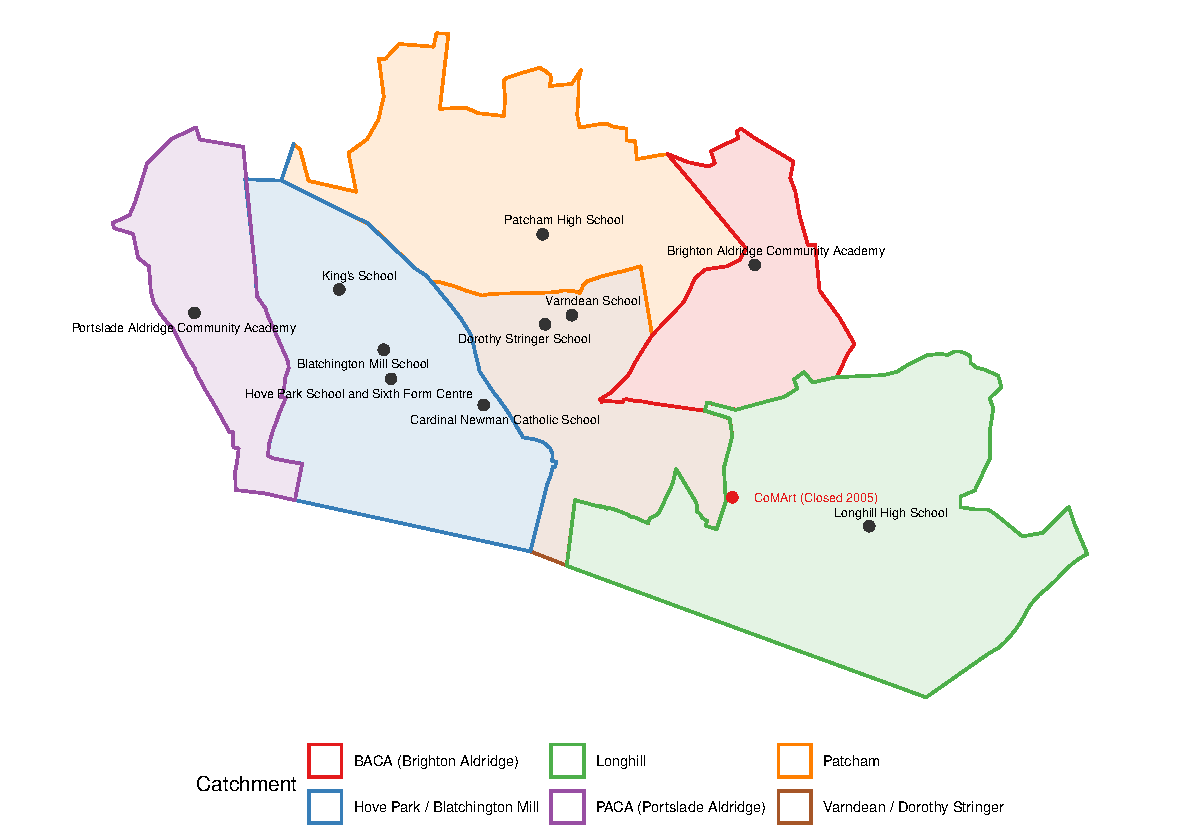
\includegraphics[keepaspectratio]{pulling_the_wrong_lever_files/figure-pdf/fig-catchments-1.pdf}}

}

\caption{\label{fig-catchments}Brighton \& Hove secondary schools with
2025/26 catchment boundaries. Click a logo or marker to see the school
name.}

\end{figure}%

As one of us has written elsewhere\footnote{\url{https://github.com/adamdennett/quarto-gisruk-2025/blob/main/DennettGISRUK2025.pdf}},
as a result of this unique admissions landscape, Brighton and Hove has
been something of a curiosity case study for education-focused
journalists and academics over the years (Allen et al., 2013; Millar,
2017). The Council is the admission authority for the community schools
in Brighton and Hove (a rare example of a local authority where 60\% of
the secondary schools in the city are still under direct LEA control),
and is required by section 88C of the School Standards and Framework Act
1998 (``the SSFA 1998'') to determine its admission arrangements in
advance of each school year. Under these rules it also has a statutory
duty to consult with the public on any changes it wishes to make. In
October 2024, it launched a public engagement exercise where they
solicited opinions from parents and other concerned parties on proposals
to further evolve secondary school admissions in the city which was then
followed by a full consultation a few weeks later.

Following the local elections in May 2023, the Labour Party took overall
control of the council in the city (where previously no single party had
commanded overall control and the Greens and Labour vied for political
superiority) and in May 2024 implemented a Leader and Cabinet system,
shifting decision making away from a distributed cross-party committee
system, to a more centralised executive structure, meaning through a
whipped voting system, party policy could be enacted without opposition
amendments. While the council has a statutory duty to consult with the
public on school admissions, it is not bound by the outcomes. And where
one party has overall control and the scope for external amendments
limited, unpopular policy can still be enacted.

The initial proposals included reducing Pupil Admission Numbers (PANs)
at some schools in the city and redrawing catchment
boundaries\footnote{Initial proposals can be seen in the papers for the
  People Overview and Scrutiny Committee held on 9th October 2024, here
  ---
  \url{https://democracy.brighton-hove.gov.uk/ieListDocuments.aspx?CId=1129&MId=11719&Ver=4}}
--- the response to this from the city was overwhelmingly
negative\footnote{\url{https://yourvoice.brighton-hove.gov.uk/en-GB/projects/secondary-school-engagement-exercise}}
with the summary of the feedback from the council stating ``\emph{While
there was broad agreement about the importance of maintaining thriving
schools and ensuring educational equity, significant concerns were
raised about the proposed methods for achieving these goals. The
feedback revealed a strong preference for improving existing schools
rather than redistributing students, alongside deep concerns about
potential impacts on community cohesion and student wellbeing}''.
However, when the statutory consultation was launched, the proposals had
been amended but the redistribution of students was still a central
pillar of the proposals and included new admissions priorities with a
proposal to reserve 20\% of places in some central schools for children
from outside of these catchments\footnote{Final proposals following the
  initial engagement exercise can be viewed in the papers for the
  Cabinet meeting held on Thursday 5th December 2024, here ---
  \url{https://democracy.brighton-hove.gov.uk/ieListDocuments.aspx?CId=1110&MId=11613&Ver=4}}.

The council's stated aims in the published papers were to improve
educational outcomes for disadvantaged pupils and to ensure that all
secondary schools in the city were viable in the face of a projected
future decline in the overall numbers of students in the city and
varying popularity in terms of applications. There was also a stated
assumption that the council believed that attainment in the city was
primarily ``driven by economic advantage''. The final proposals in the
consultation saw a key catchment boundary change in the east of the city
and reductions in overall places available at two of the most popular
and oversubscribed schools (Blatchington Mill and Dorothy Stringer).
Fewer places would be available for children living in central
catchments as 20\% of the remaining places (after PAN reductions) would
be reserved for out of catchment children ahead of in-catchment
children. The outcome of these combined policy decisions (effectively
reducing available places for in-catchment children within the Varndean
and Dorothy Stinger catchment by 150) would be to force children
(beginning from 11 years of age) from the central catchments to attend
under-subscribed schools at the periphery of the city, potentially
requiring over 2 hours of commuting on public transport per day. While
useful for the council balancing budgets, this was not popular with
those parents whose children faced being unable to attend their local
school.

At this point we will set aside the torrent of objections from parents,
loud enough to appear in the national print media\footnote{\url{https://www.thetimes.com/uk/education/article/brighton-school-admissions-shake-up-a-war-on-middle-class-families-6lbd9bjcd}
  and
  \url{https://www.telegraph.co.uk/money/jobs/schools-universities/radical-labour-council-class-warfare-south-coast/}}
and focus on the evidence-base used to justify the policy decisions in
the first place. From the papers accompanying proposals put forward, as
well as the content of the council's People Overview and Scrutiny
Committee meeting held on 9th October 2024, it is clear that the council
had settled on an attempt to affect increased mixing of disadvantaged
and non-disadvantaged students in its secondary schools --- beyond the
high levels of mixing already present (the LEA is in the top third
already for the integration of disadvantaged and non-disadvantaged
students in its secondary schools\footnote{\url{https://adamdennett.github.io/BH_Schools_Consultation/absence.html}})
--- in the belief that this would raise disadvantaged attainment. The
proposals put out for consultation at the end of 2024 were in addition
to a policy change the previous year that gave students eligible for
Free School Meals priority over most other students (both in- and
out-of-catchment) in the event of a tie-break over available places ---
a policy which went through without objection in the city and one which
was already working to affect further social mixing in schools. By
reducing the numbers of places available at popular schools in the
centre of the city --- combined with an out-of-catchment priority for a
number of students --- the policy had another, but poorly articulated
benefit for the local authority. If parents agreed to send their
children on this commute then filling under-subscribed schools on the
geographic periphery of the city, it would support these schools to
remain financially viable. That the central catchments were perceived to
be more `middle-class' and the peripheral schools in the East of the
city (in particular) perceived to be more `working-class' may have also
factored into this policy design.

We won't be able to answer in this paper whether the availability of a
more accessible evidence-base would have led to different policy
decisions from the council --- it may have done, but equally may not
have. All policies like this are entangled with political ideology and
if the broad evidence consensus doesn't align with strongly-held
political convictions then this evidence can be easily ignored or
selectively treated. But having been on the side of the city responding
to consultation proposals rather than generating them, we are able to
say that a more accessible evidence-base \emph{would} have made it
easier to engage constructively and at an earlier point in proceedings
than we were afforded given the rush to push this particular policy
through. Earlier engagement with compelling evidence may have allowed
parents, schools and councillors from all political parties to challenge
the policies with more certainty or open up more constructive lines of
critical public discussion around the drivers of attainment and the
experience of disadvantaged students in the city relative to those
elsewhere in the country.

Accessible evidence would have also been useful in challenging negative
representations of certain schools based largely on crude attainment
statistics and out-of-date Ofsted reports along with beliefs about the
benefits or otherwise of sending children to schools on the other side
of the city to their homes. And it will have allowed for more informed
questions to have been asked of experts in the scrutiny committee
meetings. Professor Stephen Gorard, appeared as an expert witness for
the council in the 9th October 2024 People Overview and Scrutiny
Committee meeting and commented that there would be ``no
losers''\footnote{Section 13.3 of the published minutes of the People
  Overview and Scrutiny Committee Meeting, 9th October 2024 ---
  \url{https://democracy.brighton-hove.gov.uk/ieListDocuments.aspx?CId=1129&MId=11719&Ver=4}}
by de-clustering disadvantaged students in the city's schools. He
conceded that he wasn't commenting on the specific BHCC proposals, but
the general point was that there were no negative effects from
increasing the proportion of disadvantaged pupils at highly performing
schools with low-levels of disadvantage. However, a better understanding
of the city's existing levels of clustering/integration and the relative
trade-offs where longer journeys might exacerbate issues like absence
(see Thomson, 2023) --- a particularly acute problem for the city as we
will see shortly --- would have facilitated much more effective scrutiny
of the policy proposals. And importantly the council made its own
interpretation of this and placed considerable weight on evidence that
was not necessarily relevant for the particular situation in Brighton
and Hove.

It's clear from the literature review above that segregation and
concentrations of disadvantage are just one of many factors contributing
to educational attainment. And it is also clear from the recent
experience in Brighton and Hove that despite the wealth of literature
out there, timely, accessible and context-relevant evidence for councils
making policy and schools and parents responding to it, is not readily
available. One of the issues is, despite each of the studies reviewed
above (and many more besides) existing, it's incredibly hard to
disentangle the relative importance of these different factors from each
other and apply them to specific local contexts. In the Brighton and
Hove case, yes, there is evidence from scholars such as Professor
Gorard, which points to the impact of social mixing and disadvantaged
segregation on attainment, but there is also a wealth of evidence on a
whole range of other factors such as attendance or low prior attainment.
The challenge for policy makers and consultation responders alike is in
how we disentangle these factors and judge their relative importance,
not just in general terms, but in the terms that relate to the very
specific local geographic contexts that present themselves in different
Local Education Authorities. Is there evidence that is easy to hand?
Evidence in addition to that tucked away in the National Pupil Database
--- an admittedly fantastic resource, but one which no-one can access
rapidly --- and which schools and parents under pressure to respond
rapidly to policy proposals can make use of?

In the remaining sections of this paper we hope to demonstrate that
there \emph{is} evidence that is easy to access, that \emph{can} be
accessed quickly and that \emph{can} shine a light on both general
drivers of attainment and specific local situations. This evidence can
be incredibly useful for both disentangling effects, but also for more
effectively benchmarking schools and helping understand the relative
impacts of different policy levers in different local situations.

We will present a model which predicts Attainment 8 for all pupils,
disadvantaged pupils and non-disadvantaged pupils, at the school level
in England, using four years of annual data. We are not claiming that
this model is the best model that can be achieved or that the particular
variables we select are the best we could have selected. Our intention
is to show that with open, freely available data from the Department for
Education, and variables that are along the right lines, it's possible
to build an incredibly accurate model of school-level attainment that in
many cases predicts well over 80\% of the variation in attainment scores
with just a handful of variables. This is useful as when we know the
vast majority of influences on attainment and how they come together and
interact in different local contexts, we can answer questions like `is
attempting to change the social mix in Brighton and Hove's Schools,
likely to have the desired impact on disadvantaged attainment' or `what
is the most important factor affecting attainment of disadvantaged
pupils in Brighton and Hove?' or `which schools are doing better or
worse than we would expect, compared to their peers nationally, or
within the city?'. We will show how not only can we answer these
questions but we can present the effects not just in statistically
correct (but widely unintelligible) standard deviations, but
policy-relevant GCSE points. To our knowledge, no openly available tool
exists that would help stakeholders develop this understanding, so we
present our efforts and welcome ideas and suggestions to improve it. We
will conclude with some reflections on our particular local case study
and the wider implications for education policy at the local level in
England.

\section{Department for Education Open
Data}\label{department-for-education-open-data}

In England, the Department for Education publishes vast amounts of open
data on schools and their key characteristics via its website ---
\url{https://get-information-schools.service.gov.uk/}. Performance,
absence and pupil population data are available from here:
\url{https://www.compare-school-performance.service.gov.uk/}, while a
potpourri of other data on aspects such as finance and funding, teachers
and school workforce, as well as additional data on pupils, schools and
their outcomes are all available via the explore education statistics
service --- \url{https://explore-education-statistics.service.gov.uk/}.

The publication schedule for these open datasets varies with annual
revisions for performance, finance and workforce statistics, whereas
increasingly, absence and attendance statistics are now reported with
much higher temporal regularity, at the cost of some spatial granularity
(school level statistics only available termly and yearly).

These data provide an incredibly rich --- and in our view, underutilised
--- source of data on schools and their drivers of attainment. They are
relatively consistent over time and in the analysis we present below, we
will cover the last 4-years of statistics from 2021-22 through to
2024-25 --- the immediately post-COVID and post-imputed grade period
(Prior and Leckie, 2025).

Data-pre-processing (linkage, cleaning, imputation) was required to
complete a consistent, harmonised 4-year time-series. The details of
this are available in the
\href{https://adamdennett.github.io/school_attainment_tool/data_overview.html}{supplementary
material}\footnote{\url{https://adamdennett.github.io/school_attainment_tool/data_overview.html}}.
At the end of the pre-processing stage, we have an analysis full panel
of 13,419 school-year observations from 3523 academies and maintained
schools across 152 Local Education Authorities in England over 4
academic years (2021--22 to 2024--25). Independent schools, colleges and
special schools are excluded from this analysis. All processed data used
can be downloaded from
\href{https://drive.google.com/drive/folders/1PWdJVELz5IsU7ASa5ZuCez8ypkyrd0CK?usp=sharing}{here}\footnote{\url{https://drive.google.com/drive/folders/1PWdJVELz5IsU7ASa5ZuCez8ypkyrd0CK?usp=sharing}}
with all processing code available
\href{https://github.com/adamdennett/school_attainment_tool/tree/main/R}{here}\footnote{\url{https://github.com/adamdennett/school_attainment_tool/tree/main/R}}.

We should reiterate that all data used in this analysis are school-level
and not pupil-level. Therefore any interpretations relate to this level
of aggregation. This is important as nothing we observe here should be
taken to apply to individual pupils in isolation, rather the averages
across all similar pupils in a school and then between schools. Where we
will go on to make reference to general patterns and trends related to
disadvantaged and non-disadvantaged pupils, it is, of course, the case
that there will be individuals who behave very differently to the
average. But where policies are made at this more aggregate school
level, we believe this is entirely appropriate.

\section{Modelling School Level
Attainment}\label{modelling-school-level-attainment}

Effective pupil attainment policies need to understand the relative
influence of different causal factors and their confounding and
mediating interactions. In our Brighton and Hove case study, the
attention of the policy makers in 2024 was almost entirely focused on
the effects of disadvantage on attainment --- an important variable, but
as we shall see, one that should not be looked at in isolation where
confounding and mediating variables such as absence and low prior
attainment play an important role.

Our modelling here is undertaken with a number of key objectives in
mind. We want to understand:

\begin{itemize}
\tightlist
\item
  the impacts of non-linear relationships between variables and what
  these mean for different schools and local authorities
\item
  how good these school level models are --- how much is attainment
  predictable in the context of other readily available information
  about schools?
\item
  the relative importance of different factors influencing variation in
  attainment across schools and over space and time and their
  confounding and mediating influences on each other
\item
  what different policy scenarios might mean in terms that make
  intuitive sense to policy makers, school leadership and parents ---
  attainment 8 / GCSE points, rather than standard deviations
\item
  how we might be able to benchmark schools differently in the context
  of better attainment models
\item
  how this information, if available at the time, could have been used
  to inform the debate in Brighton and Hove during the 2024 consultation
  --- and how it might be used to fill the information vacuum in future
  both in other local situations and in national debates.
\end{itemize}

To reiterate, in this exercise we are not trying to build the most
accurate model possible or reveal previously unknown truths --- the
model we present can certainly be refined and many of the associations
between drivers and outcomes well established. Where the Brighton and
Hove situation demonstrated there was a big gap, however, was in
synthesising and assessing the relative contributions of the factors
impacting secondary school attainment and relating these to specific
local contexts. We hope to demonstrate that it's possible to build a
very good model or suite of models --- good enough to explain most of
the variation in Attainment 8 across schools in England --- from just a
small selection of readily available and up-to-date variables. And these
can be used to gain important policy-relevant insights that are specific
to the unique local situations experienced across all LEAs in England.
The explanatory variables we selected are shown in
Table~\ref{tbl-variables} below.

\begingroup\fontsize{11}{13}\selectfont

\begin{longtable}[t]{lrrrrrrr}

\caption{\label{tbl-variables}Model Outcome and `Fixed Effect'
explanatory variables used in the model.}

\tabularnewline

\toprule
Variable & N & \% available & Mean & SD & Min & Median & Max\\
\midrule
\addlinespace[0.3em]
\multicolumn{8}{l}{\textbf{Outcome}}\\
\hspace{1em}Avg. Attainment 8 score per pupil & 12210 & 100.0 & 47.64 & 9.40 & 0.80 & 46.50 & 88.20\\
\hspace{1em}Avg. Attainment 8 score (disadvantaged) & 12071 & 100.0 & 38.52 & 9.46 & 12.90 & 36.90 & 86.00\\
\hspace{1em}Avg. Attainment 8 score (non-disadvantaged) & 12071 & 100.0 & 50.43 & 8.29 & 11.20 & 49.50 & 87.50\\
\addlinespace[0.3em]
\multicolumn{8}{l}{\textbf{School composition}}\\
\hspace{1em}\% KS4 pupils who are disadvantaged & 12210 & 100.0 & 26.93 & 14.38 & 0.60 & 24.40 & 96.00\\
\hspace{1em}\% overall absence & 12210 & 100.0 & 8.86 & 2.49 & 2.03 & 8.70 & 28.10\\
\hspace{1em}\% pupils with English not first language & 12210 & 100.0 & 18.06 & 18.49 & 0.20 & 10.80 & 94.80\\
\hspace{1em}\% KS4 pupils with low prior attainment (KS2) & 12199 & 99.9 & 22.84 & 10.20 & 0.00 & 22.70 & 92.00\\
\hspace{1em}Admissions policy (new definition from 2019) & 12210 & 100.0 & NA & NA & NA & NA & NA\\
\addlinespace[0.3em]
\multicolumn{8}{l}{\textbf{Segregation (LA-level)}}\\
\hspace{1em}Gorard segregation index & 12210 & 100.0 & 0.17 & 0.05 & 0.00 & 0.17 & 0.32\\
\addlinespace[0.3em]
\multicolumn{8}{l}{\textbf{Workforce}}\\
\hspace{1em}Teachers remaining in same school (FTE) & 12210 & 100.0 & 54.37 & 21.19 & 1.00 & 52.60 & 155.90\\
\hspace{1em}\% teachers on leadership pay range & 12210 & 100.0 & 11.72 & 4.84 & 0.00 & 10.91 & 66.67\\
\hspace{1em}Avg. teacher sickness days & 12210 & 100.0 & 8.28 & 3.52 & 0.10 & 7.80 & 91.50\\
\bottomrule

\end{longtable}

\endgroup{}

Our model is an extension of a standard linear regression model known as
a linear mixed effects model --- and in this case we use a multi-level
specification where we have schools nested within LEAs which exist
within wider English Regions. Linear mixed effects models (LMEs) offer
several advantages over standard ordinary least squares (OLS) regression
when data have this hierarchical or nested structure (Snijders, 2012).
For example, OLS regression assumes that all observations are
independent, an assumption that is violated when individuals share a
common context --- pupils within the same school, for instance. We are
not analysing pupil-level data, but in our example, schools within LEAs
/ regions or within the same Ofsted grade banding or assessment year
might be more similar to each other within rather LMEs address this by
explicitly modelling the variance at each level of the hierarchy through
the inclusion of these grouping variables or `random effects'. The
effect is more correctly-adjusted standard errors and more reliable
inference.

The choice of main explanatory `fixed-effects' was informed by the
various studies mentioned in the earlier review, as well as by the
narrative that emerged from the Council during the consultation in
Brighton and Hove. In this case, significant prominence was given to the
segregation and work of Professor Stephen Gorard. Indeed as mentioned,
he gave evidence at the People Overview and Scrutiny Committee. As such
we have included a derived Gorard Segregation Index variable here for
comparison with other variables including levels of disadvantage,
absence, prior attainment, English not as a first language, teacher
retention, teacher sickness and senior leadership and a dummy variable
for non-religious admissions selectivity. Random effects included
observation year (for the full panel model), 4-category Ofsted rating
(harmonised to the more recent 4 category scheme), Government Office
Region and Local Education Authority nested within that region.

The final full panel model for overall Attainment 8 can be written as:

\[
\log(\text{ATT8}_{ij}) = \beta_0 + \sum_{k=1}^{9} \beta_k \, x_{kij} + u_{\text{year}} + u_{\text{Ofsted}} + u_{\text{region}} + u_{\text{LA|region}} + \varepsilon_{ij}
\]

where \(i\) indexes schools, \(j\) indexes year observations, the
\(\beta_k\) are fixed-effect coefficients, and the \(u\) terms are
random effect intercepts. Because the outcome is on the \emph{log
scale}, each coefficient represents the proportional change in
Attainment 8 associated with a one-unit change in the predictor (or, for
log-transformed predictors, an \emph{elasticity} --- the percentage
change in ATT8 for a 1\% change in the predictor). We fit this model
using the \texttt{lme4} package in R.

We fit several different versions of this model --- details of which can
be found in the
\href{https://adamdennett.github.io/school_attainment_tool/model_experiments.html}{supplementary
material}\footnote{\url{https://adamdennett.github.io/school_attainment_tool/model_experiments.html}}
--- but which can be broken down into the following classes:

\begin{itemize}
\tightlist
\item
  A Panel model which includes all four years of data with year as an
  additional random effect (final versions including some imputed data
  for 2024-25)
\item
  Individual year models for each of the 2021-22, 2022-23, 2023-24 and
  2024-25 years.
\item
  Each of these are run for overall Attainment 8 across all pupils, but
  then also for Attainment 8 for disadvantaged and non-disadvantaged
  pupils separately.
\end{itemize}

\subsection{Non-linear Effects}\label{non-linear-effects}

The crucial policy message for non-linear effects is: context matters.
Where you are on an effect distribution can make a big difference. And
in a city like Brighton and Hove, with levels of disadvantage close to
the national average in most schools (and significantly above in two),
all other things being equal (and we will come to this shortly), even
fairly big shifts in levels of disadvantage (moving all schools to the
city average, for example) are unlikely to have a big impact on
attainment at the school level.

Take Figure~\ref{fig-bivariate-raw} below which plots every school over
the entire period with All Pupil Attainment 8 on the Y axis and the \%
of Disadvantaged Students in a school on the X axis. Above about 20\%
disadvantaged students (the national average being around 27\% over this
period), further increases in disadvantage do not correlate with
noticeable further declines in Attainment 8. Put another way, halving a
school's FSM proportions from around 55\% to the national average would
be unlikely to result in a big increase in attainment. Indeed most of
the strong effect appears to be at the low end of disadvantage, below
about 15\%, where further reductions are correlated with a much steeper
increase in Attainment 8. The red line is the OLS linear regression
line, but it shows a straight line is not a good approximation of the
relationship.

\begin{figure}

\centering{

\pandocbounded{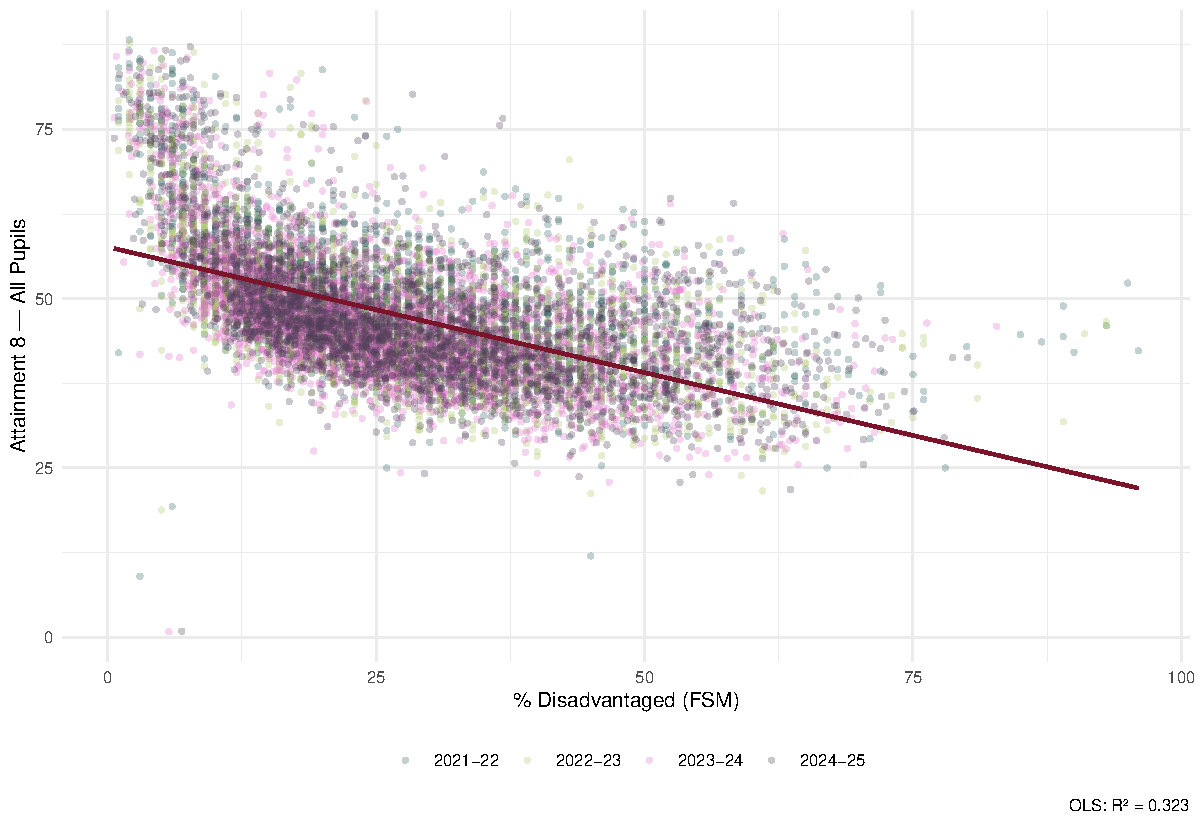
\includegraphics[keepaspectratio]{pulling_the_wrong_lever_files/figure-pdf/fig-bivariate-raw-1.pdf}}

}

\caption{\label{fig-bivariate-raw}Bivariate correlation between
School-Level Attainment 8 and \% Disadvantaged Children. Each point is a
school-year observation; the red line is the OLS fit.}

\end{figure}%

This curved relationship can be flattened and made linear by taking the
log of both variables. See Figure~\ref{fig-bivariate-log} below. The
log-log relationship is linear and this is useful for our linear models,
but perhaps less well appreciated is what this means in practical policy
terms. Stating that as concentrations of disadvantage increase,
attainment decreases is both true and misleading at the same time. The
strength of the relationship is entirely dependent on where in the
distribution a school sits. A detailed account of this can be found in
the
\href{https://adamdennett.github.io/school_attainment_tool/brighton_case_study.html\#sec-nonlinear}{supplementary
material}\footnote{\url{https://adamdennett.github.io/school_attainment_tool/brighton_case_study.html\#sec-nonlinear}},
but in short a log-log relationship is an elasticity which means that
percentage changes are linear but percentage changes at one end of the
distribution have far more or less impact than at the other.

\begin{figure}

\centering{

\pandocbounded{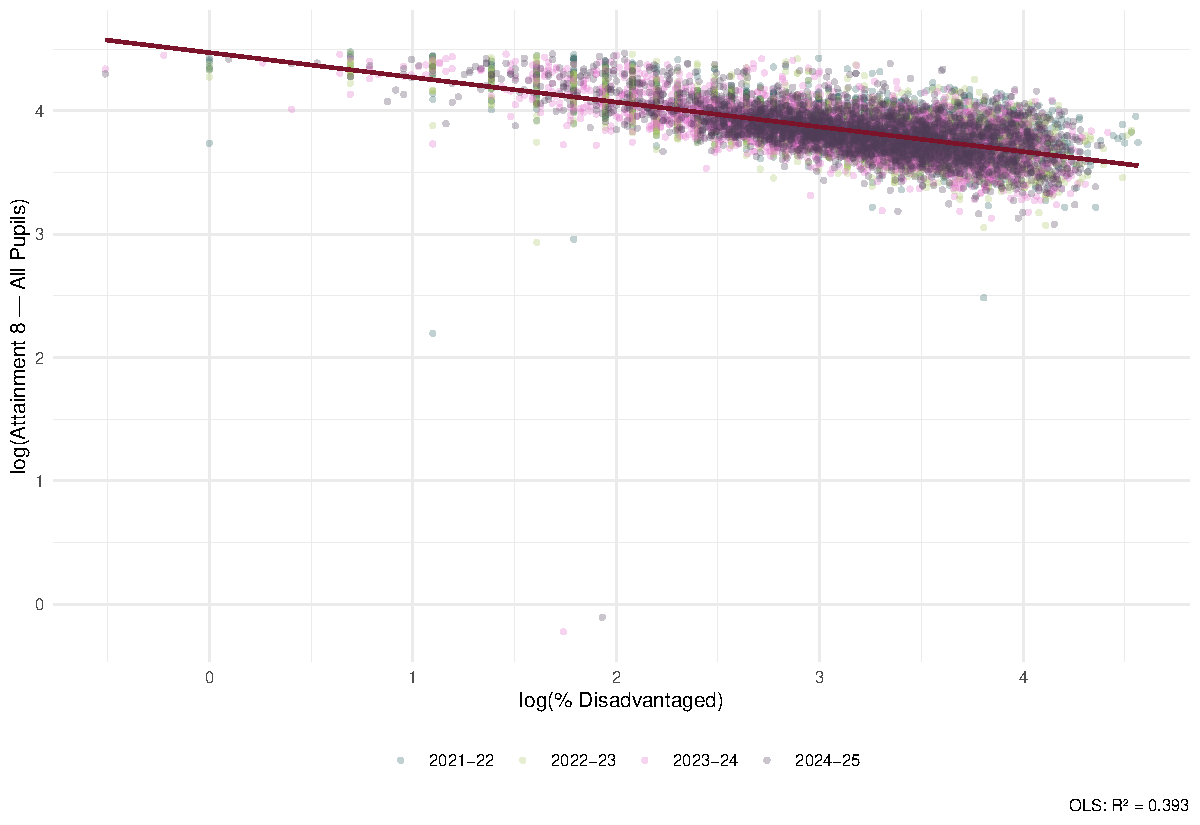
\includegraphics[keepaspectratio]{pulling_the_wrong_lever_files/figure-pdf/fig-bivariate-log-1.pdf}}

}

\caption{\label{fig-bivariate-log}Log-log bivariate correlation between
School-Level Attainment 8 and \% Disadvantaged Children. The log
transformation linearises the relationship, revealing the elasticity.}

\end{figure}%

As we also detail in the
\href{https://adamdennett.github.io/school_attainment_tool/data_overview.html\#bivariate-relationships}{supplementary
material}\footnote{\url{https://adamdennett.github.io/school_attainment_tool/data_overview.html\#bivariate-relationships}},
non-linear associations are found between Attainment 8 (all,
disadvantaged and non-disadvantaged) and most of the predictor variables
in the model. To re-iterate, these non-linear relationships across all
schools and years mean that individual local authorities need to
carefully consider where each school lies on the scale across these
different variables to fully appreciate what impacts changes in the
values of these variables might mean for a particular school or
collection of schools.

\subsection{How good are the models?}\label{how-good-are-the-models}

These models are excellent in that they account for somewhere around
80\% (as evidenced by the Conditional --- fixed-effects + random effects
--- R-Squared values across the full panel and annual models\footnote{\url{https://adamdennett.github.io/school_attainment_tool/model_results.html\#model-fit-comparison-across-years}})
of the variation in Attainment 8 for all pupils. The fits for
disadvantaged pupils are slightly worse than they are for
non-disadvantaged pupils, signifying the additional variation in
disadvantaged student attainment caused by other external factors not
measured, but with R-squared values around 70\%, in a social science
context with all of the noise inherent in human systems, it would be
difficult to find models explaining this much variation in an outcome
variable. Attainment at the school level is incredibly predictable.

That these models explain such a high proportion of the variation in
attainment is crucially important in policy terms as it means if we know
what causes higher or lower attainment across these different groups of
students, it's possible to choose more targeted interventions that are
likely to have more significant impact. It also means that the
conversation around the efficacy or otherwise of proposals can be better
informed by what we know about both the national evidence-base and more
specialist knowledge of local conditions.

\subsection{What do the Models reveal? Results and
Interpretations}\label{what-do-the-models-reveal-results-and-interpretations}

\begin{table}

\caption{\label{tbl-stepwise}Step-wise Progression to Full 4-year
Imputed Panel Model with Fixed + Random Effects.}

\centering{

\centering\begingroup\fontsize{8}{10}\selectfont

\begin{tabular}[t]{lrlrlrlrlrl}
\toprule
\multicolumn{1}{c}{ } & \multicolumn{2}{c}{Model 1: FSM only} & \multicolumn{2}{c}{Model 2: + Absence} & \multicolumn{2}{c}{Model 3: + Prior att.} & \multicolumn{2}{c}{Model 4: All fixed} & \multicolumn{2}{c}{Model 5: Full multilevel} \\
\cmidrule(l{3pt}r{3pt}){2-3} \cmidrule(l{3pt}r{3pt}){4-5} \cmidrule(l{3pt}r{3pt}){6-7} \cmidrule(l{3pt}r{3pt}){8-9} \cmidrule(l{3pt}r{3pt}){10-11}
Variable & Est. & t & Est.  & t  & Est.   & t   & Est.    & t    & Est.     & t    \\
\midrule
(Intercept) & 4.473*** & 621.25 & 5.006*** & 579.97 & 4.833*** & 547.18 & 4.628*** & 319.11 & 4.633*** & 125.61\\
log(% FSM) & -0.201*** & -88.94 & -0.122*** & -59.66 & -0.073*** & -33.46 & -0.071*** & -28.60 & -0.067*** & -24.90\\
log(% Absence) &  &  & -0.364*** & -82.87 & -0.287*** & -65.28 & -0.242*** & -51.65 & -0.213*** & -46.03\\
log(% EAL) &  &  &  &  &  &  & 0.014*** & 13.69 & 0.006*** & 4.92\\
% Low Prior Attainment &  &  &  &  & -0.006*** & -45.75 & -0.005*** & -37.59 & -0.006*** & -41.35\\
Admissions: Other non-selective (ref: non-sel. in highly sel. area) &  &  &  &  &  &  & 0.051*** & 11.01 & 0.001 & 0.08\\
Admissions: Selective (ref: non-sel. in highly sel. area) &  &  &  &  &  &  & 0.140*** & 19.96 & 0.108*** & 16.20\\
Gorard Segregation &  &  &  &  &  &  & 0.052 & 1.92 & -0.033 & -0.69\\
Teacher Retention &  &  &  &  &  &  & 0.001*** & 12.92 & 0.000*** & 10.20\\
Leadership Pay % &  &  &  &  &  &  & -0.001*** & -6.10 & -0.001*** & -5.39\\
log(Teacher Sickness) &  &  &  &  &  &  & -0.016*** & -6.08 & -0.015*** & -6.17\\
Random effects &  &  &  &  &  &  &  &  &  & \\
LA (nested in region) &  &  &  &  &  &  &  &  & 0.030 & (SD)\\
Region &  &  &  &  &  &  &  &  & 0.017 & (SD)\\
Ofsted rating &  &  &  &  &  &  &  &  & 0.047 & (SD)\\
Year &  &  &  &  &  &  &  &  & 0.044 & (SD)\\
Residual &  &  &  &  &  &  &  &  & 0.094 & (SD)\\
 &  &  &  &  &  &  &  &  &  & \\
R² & 0.3932 &  & 0.6117 &  & 0.6686 &  & 0.6929 &  & 0.6319 & (marginal)\\
R² (conditional) &  &  &  &  &  &  &  &  & 0.7712 & (fixed + random)\\
N & 12,210 &  & 12,210 &  & 12,210 &  & 12,210 &  & 12,210 & \\
\bottomrule
\end{tabular}
\endgroup{}

}

\end{table}%

\subsubsection{Full Model}\label{full-model}

The relative importance of the variables and their contribution to the
overall story can be observed through the stepwise progression through 5
models shown in Table~\ref{tbl-stepwise}. In this table. Model 1 on the
left of the table is the most simple bivariate model --- also shown in
Figure~\ref{fig-bivariate-log}. Models 2 and 3 then add absence and low
prior attainment variables with the changes in the coefficients showing
first the mediating effect of absence and then the additional mediating
impact of low prior attainment while both push the explanatory power of
the model up significantly. Models 4 and 5 add additional fixed and then
finally random effects into the explanatory mix.

Mediating variables sit along the causal pathway between a predictor and
an outcome. Part of the reason why deprived pupils have lower attainment
is because deprivation often leads to higher rates of unauthorised
absence (due to health, transport, or family circumstances etc.), and
that absence then leads to lower grades. In Model 1, levels of
deprivation --- proxied by the \% of students on Free School Meals ---
is significant and negatively impactful on school-level attainment 8.
When you add log(\% Absence) in Model 2, the \%FSM coefficient shrinks
dramatically, almost halving from -0.201 to -0.122. In effect, absence
``stole'' a large chunk of the explanatory power from deprivation.

When you add Prior Attainment at KS2, both the FSM and Absence
coefficients shrink again (FSM goes from -0.122 to -0.073, absence from
-0.364 to -0.287). There could be an argument that low prior attainment
confounds some of the effects of absence on attainment (in some cases,
it could be a common cause of both), however both low prior attainment
and absence act as mediators sitting between deprivation and attainment
outcomes. We are not claiming revelatory insights here around the impact
of prior attainment --- indeed this is exactly why measures like
Progress 8 have existed for a long time --- but in this context of
policies being shaped around deprivation without a parallel conversation
around absence and low prior attainment, it's useful to acknowledge the
extent to which without accounting for these two important mediating
variables --- something entirely absent from the council policy
proposals and consultation narrative in Brighton and Hove --- the
importance of deprivation, while still a factor, is less important on
its own. A fact that could lead to misdirected and potentially damaging
(for attainment across the city) policy decisions.

By Model 3, with just three variables, we are already accounting for
two-thirds of the variation in attainment across schools in England.
Examining the standardised coefficients (t-values = coefficient /
standard error) gives an indication of the relative importance of each
variable in the story --- larger positive or negative values giving a
sense of relative importance (although strictly, standardised
coefficients --- coefficient × standard deviation --- are a better
measure). With t = -65.28, absence is doing most of the heavy-lifting
and nearly double the t-value for deprivation. Low prior attainment (t =
-45.75) is the next most important variable in the story, confirming the
idea that a large amount of the variation in attainment at age 16
explained by the levels of attainment pupils arrive at secondary school
with. In this three variable model, there is still an important residual
poverty effect. The proportion of deprived pupils in a school (t =
-33.46) that remains after we account for absence and prior attainment
is still significant suggests at this stage that deprivation is an
ongoing hindrance for attainment. However, there might be additional
variables which add to the story and these are explored in models 4 and
5.

Model 4 adds some additional variables including the proportion of
pupils in a school with English as an additional language, selective
admissions (a dummy variable) and a suite of teaching and leadership
variables including teacher retention, sickness and leadership pay. All
of these suppress the effects of the deprivation, low prior attainment
and absence triad, reflecting to a degree a school-level institutional
buffer whereby staff stability can mitigate some of the negative effects
noted earlier.

Model 5 is the full specification with additional grouping factors
(random effects) including geographical location (Local Education
Authorities within Regions) the Ofsted\footnote{\url{https://www.gov.uk/government/organisations/ofsted/about}}
rating of the school and year of analysis (in this full 4-year panel
model). These random effects add a considerable amount of additional
power to the model with a shift in R-squared from 0.63 (Marginal) to
0.77 (Conditional) indicating that 14\% of the variance in school-level
attainment 8 is tied to these ``Random Effects''. It's important to note
in this full model specification that while many of the fixed effects
will contribute to whether a school is judged `outstanding' or `requires
improvement' with all variables in the model, these grouping factors are
capturing some of left over effects --- the `residual variance' in
statistical terms. In terms of Ofsted rating, these might be things like
the culture and leadership within the school, teaching quality, or
behaviour management policies. In terms of the geographical random
effects these could be community factors within local authorities,
school leadership and governance within a local authority, effective
school-to-school collaboration networks or effective local authority led
school improvement programmes.

Before commenting on some important differences between this overall
model and sub-models for disadvantaged and non-disadvantaged attainment
specifically, it's worth noting that the local authority level Gorard
Segregation variable is not statistically significant in either Model 4
or 5. Once you account for a school's own FSM levels, its students'
prior attainment, their attendance, and the region they are in, the
specific ``clustering'' of disadvantaged students in schools within a
local authority doesn't seem to add any extra predictive power to the
school's results. We include it in this model as school segregation
arguments formed much of the justification for the council admissions
proposals in Brighton and Hove in 2024. This evidence doesn't
necessarily contradict expert opinion given to the council as
segregation \emph{could} lead to higher absence (perhaps due to peer
effects) or lower teacher retention (perhaps due to more challenging
working conditions), but any harm that segregation might cause is
already fully mediated by the variables already included in the model.
The flipping of the Gorard Segregation coefficient between Models 4 and
5 could be due to some highly segregated LEAs, like those in London,
having very high levels of attainment, which once controlled for in the
multilevel model, leave the variable with no more explanatory power to
contribute. Where the expert evidence could be criticised in this
instance is in ignoring the big issues of absence in the city and
failing to highlight that this is a more pressing issue and impactful
policy lever.

\subsubsection{Disadvantaged and Non-Disadvantaged
Attainment}\label{disadvantaged-and-non-disadvantaged-attainment}

Perhaps the most contentious observation that the school-level modelling
reveals is that across all schools in England over the 4-years studied,
disadvantaged pupils actually perform slightly better when they are at
schools with higher concentrations of other disadvantaged pupils,
provided they attend school and once we account for other factors like
prior attainment. This will be a controversial observation in the
context of the policy narratives in our case study city and in relation
to the evidence presented by Professor Gorard at the People Overview and
Scrutiny Committee in October 2024, but one that is robust to different
dimensions of disadvantaged attainment and conceptions of school-level
disadvantage concentration\footnote{\url{https://adamdennett.github.io/school_attainment_tool/model_experiments.html\#sec-directionality}}.
Much of the justification for the policies consulted upon by Brighton
and Hove City Council in 2024, and eventually implemented in 2025,
centred around the belief that disadvantaged attainment could be
improved through efforts to bring all schools closer to the city Free
School Meal average through redistributing pupils across the city's
schools, and through additional efforts to constrain places in some
schools and give out-of-catchment priority to some (assumed to be more
disadvantaged) children at popular central schools. The evidence here is
that these policies are unfortunately very unlikely to improve
disadvantaged attainment and could make it worse.

One of the features of the school-level DfE data is that overall
Attainment 8 can be disaggregated by disadvantaged and non-disadvantaged
pupils as well as zooming in different aspects of the inputs to the
overall Attainment 8 statistic, including the English and Maths elements
as well as the `Open bucket'\footnote{\url{https://www.gov.uk/government/publications/progress-8-school-performance-measure/secondary-accountability-measures-2025-guidance-for-maintained-secondary-schools-academies-and-free-schools}}
elements which can include GSCEs and non-GCSEs which might be more
technical or vocational awards like BTECs and NCFE certificates.
Coefficients for the full panel models for disadvantaged and
non-disadvantaged pupils can be viewed in the
\href{https://adamdennett.github.io/school_attainment_tool/model_results.html\#disadvantaged-pupils}{supplementary
material}\footnote{\url{https://adamdennett.github.io/school_attainment_tool/model_results.html\#disadvantaged-pupils}},
but are summarised in Figure~\ref{fig-standardised-coefficients} below.

\begin{figure}

\centering{

\pandocbounded{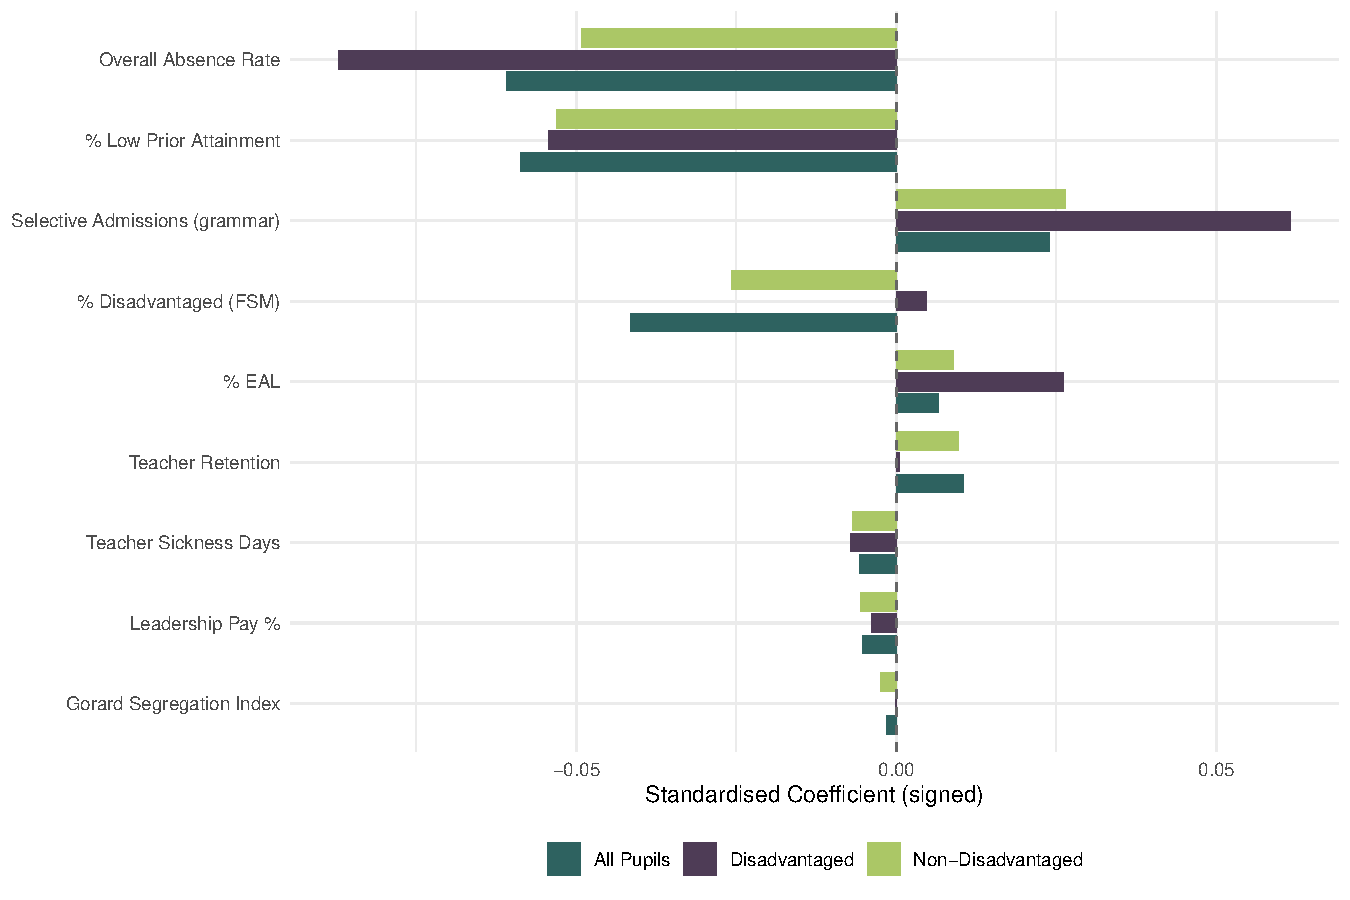
\includegraphics[keepaspectratio]{pulling_the_wrong_lever_files/figure-pdf/fig-standardised-coefficients-1.pdf}}

}

\caption{\label{fig-standardised-coefficients}Standardised coefficients:
relative variable importance across pupil groups (Model 5). Bars show
the change in log(ATT8) associated with a one-SD shift in each
predictor.}

\end{figure}%

While most predictor variables chosen have the same level and direction
of effect for all variables, the third row of bars showing the
importance of concentrations of disadvantaged pupils in schools and the
impact on Attainment 8 across the groups reveals the direction of the
effect is different for disadvantaged and non-disadvantaged pupils. The
coefficient is negative for non-disadvantaged pupils --- as the \% of
disadvantaged pupils in a school increases, Attainment 8 decreases. But
\emph{positive} for disadvantaged pupils --- as the concentrations of
disadvantaged pupils in a school increase, Attainment 8 also increases.
Across the full 4-year panel --- and in models for each individual
year\footnote{See individual year models in the supplementary material
  here ---
  \url{https://adamdennett.github.io/school_attainment_tool/model_experiments.html\#analysis-b-full-per-year-models}}
--- after controlling for all other variables in the model, but
particularly low-prior attainment\footnote{The direction of the
  coefficient for concentrations of disadvantage becomes positive in the
  presence of low prior attainment ---
  \url{https://adamdennett.github.io/school_attainment_tool/model_results.html\#disadvantaged-pupils}},
the Attainment 8 score for disadvantaged pupils increases as
concentrations of disadvantaged students also increase.

To check the robustness of this observation and to ensure it was not
just an artefact of the way that disadvantaged and non-disadvantaged
students were classified or an aspect of the qualifications included in
the overall Attainment 8 statistic such as the inclusion of vocational
or non-vocational elements, or the way in which the measure of
disadvantage we used (FSM6CLA1A --- within KS4 cohort FSM-eligible in
the past 6 years or looked-after) might have been too narrowly focused,
we ran a series of experiments to check the strength and direction of
the coefficients observed under different conceptions of disadvantaged
attainment (different Y variables) and different measures of school
level disadvantage (x-variables) --- see
\href{https://adamdennett.github.io/school_attainment_tool/model_experiments.html\#sec-directionality}{supplementary
material}\footnote{\url{https://adamdennett.github.io/school_attainment_tool/model_experiments.html\#sec-directionality}}.

While disaggregating Attainment 8 for disadvantaged pupils into its
English and Maths elements yields associations that aren't statistically
significant, focusing in on the Open element of the Attainment 8
composition shows an even stronger overall and non-GCSE sub-component
positive association with the main \% FSM variable used in the model.
Interestingly, the GCSE component of the Open element is quite strongly
negative, which is revealing. What this suggests is schools with higher
concentrations of FSM eligible pupils achieve significantly better
outcomes for disadvantaged students on more vocational/technical
pathways. This supports the specialisation argument --- these schools
with higher levels of pupil premium funding are able to invest that
money in well-targeted BTEC or other vocational programmes which may
require specialist staff or well established links to local employers
etc. --- essentially what the investment was probably originally
intended for. Some may try to argue that given the GCSE sub-component is
strongly negative, it could also reflect that better grades are more
attainable in vocational programmes --- effectively schools being able
to game their results, to some extent. However, while the GSCE Maths and
English components for disadvantaged students are not statistically
significant, the fact that Maths nudges positive is supportive of there
being a genuine effect in some GCSEs along with a clear benefit from
vocational pathways.

The full multi-level model shines further light. In Model 5, the \% FSM
coefficient drops to 0.008 and the t-value falls to 2.08 (see
supplementary material). This means that the attainment boost of being
in a higher-disadvantage school for disadvantaged pupils is largely
explained by the Region, LEA, and Ofsted rating. A disadvantaged pupil
doesn't necessarily get a boost just because the school has high levels
of disadvantage; they get a boost because higher-FSM schools in certain
LEAs or with certain Ofsted ratings (like ``Outstanding'' inner-city
schools) have mastered the art of supporting them. Once you account for
those ``Random Effects,'' the concentrations of disadvantage have almost
no remaining direct impact. This adds further weight to the
specialisation theory.

On the other hand, for non-disadvantaged pupils, the effects of higher
disadvantage are more strongly negative. Even after controlling for
their own attendance and prior scores, being in a higher-disadvantage
school depresses Attainment 8\footnote{\url{https://adamdennett.github.io/school_attainment_tool/model_results.html\#non-disadvantaged-pupils}}.
This could be a ``peer effect'' --- higher concentrations of
disadvantage in a school can correlate with disruptive behaviour
(Chazan, 2000) or it could relate to various curriculum, resourcing or
other factors.

We have acknowledged that this will be a politically contentious finding
(particularly within Brighton and Hove), so we want to make clear that
this evidence does not mean we are advocating for proactively
concentrating disadvantaged pupils in schools --- \emph{we are not}.
However what we \emph{are} saying is that where the social and spatial
structure of LEAs leads to some concentration of disadvantage in some
schools, deconcentration policies might be counter productive where
there is evidence that schools with higher concentrations of
disadvantaged pupils are able to adapt and tailor their educational
offering more effectively. Where those deconcentration policies by their
very nature mean that more students will not be attending their most
local schools and travelling on longer journeys each day, are the
negatives associated with those longer journeys (financial costs, having
to leave the home earlier in the day and return later at night, not
being able to walk to school with friends and engage in active travel,
parents more remote from the school communities, potentially higher
absence rates because of these) and their corresponding impacts on
attainment, likely to be outweighed by any benefits brought by active
deconcentration? The evidence here is that this is very unlikely.

While the \% FSM variable flips and shrinks in different contexts, the
absence variable remains consistently the biggest story and is even more
important for disadvantaged pupils than it is for non-disadvantaged
pupils. We are not overstating it to say that for disadvantaged pupils,
attendance is \emph{the most important factor} --- as is shown in
Figure~\ref{fig-standardised-coefficients}. Nearly half of the
difference in school-level performance between disadvantaged pupils is
explained simply by whether they are in the building. Concentrations of
disadvantage are a secondary concern compared to the raw impact of
missing lessons. For non-disadvantaged pupils, the impact of missing
school is nearly half as damaging as it is for disadvantaged pupils.
Disadvantaged pupils do not have the access to a safety net of engaged
parents, private tutors, revision guides that some less disadvantaged
students have, and are more reliant on the teacher in the classroom to
learn material. In some ways, attendance is the ultimate equity lever
for a school or local education authority.

There is a further element to this story. As
Figure~\ref{fig-standardised-coefficients} shows, for the few
disadvantaged pupils who make it into selective (grammar) schools (and
we can also assume independent fee-paying schools, although these are
not in our analysis), the bonus is huge. Their attainment is
significantly higher than similar disadvantaged pupils in non-selective
schools, even after controlling for their prior attainment. This could
be described as the ``Grammar School Effect''. Although given the
research cited earlier in this paper by Burgess et al. (2018), while
could be that for disadvantaged pupils, an environment with high
expectations and a high-attaining peer group might offer a boost, this
boost might be more to do with the selection bias and individual
qualities (O'Connell and Marks, 2022) of those disadvantaged students
--- against the odds (i.e.~without expensive coaching and tutoring for
the entrance exams) --- being admitted. Selective schools simply cream
off the very best students and bring them together, although whatever
the mechanism this is a much bigger effect than it is for
non-disadvantaged students.

Other teacher factors such as retention and sickness days matter, but
are very small effects in comparison. For non-disadvantaged students,
teacher stability is a highly significant predictor of success (t =
11.81). For disadvantaged students, once you control for everything
else, it actually drops out of significance (t = 0.42). This might
suggest that for students in high-poverty areas, the systems of the
school (attendance tracking, specialised FSM support) are more important
than an individual teacher staying for five years. For non-disadvantaged
students, long-term teacher relationships seem to drive more value.

English as an Additional Language (EAL \%) is also an important element
of disadvantaged attainment --- as the concentration of EAL students in
a school increases, attainment generally rises. However, when you move
to Model 5 (Multilevel), the EAL coefficient shrinks significantly (from
0.023 to 0.015 for disadvantaged pupils). It's difficult to disentangle
whether EAL is a mediator of the London (London successful because of
high aspiration EAL families) effect or the London effect is a
confounder of the EAL effect (London's better infrastructure and funding
boosting EAL student performance) or if it is a reciprocal interaction
between the two. However, in policy terms, this is not an available
lever anyway.

Apart from the specific variable effects, the model for
non-disadvantaged students is ``tighter'' (79\% of variation explained
vs 73\%). This suggests that the progress of less-disadvantaged students
is more predictable based on these structural factors while the progress
of disadvantaged students is less tightly aligned --- their success can
be more influenced by unmeasured individual resilience or specific local
interventions that we have not captured in these models.

With this evidence, the policy implications should be clear --- a focus
on attendance and mitigating the impacts of low prior attainment should
be the priorities for policy makers. Any attempts to affect attainment
through changing the proportions of disadvantaged and non-disadvantaged
students in schools are unlikely to have much impact at the school-level
and could have the opposite impact on disadvantaged students. But beyond
this what is really required for policy makers, school leaders and
parents alike, is an ability to translate these general observations to
very specific local contexts --- contexts that really matter where
schools will sit along a continuum for each of the variables that might
impact attainment and where many of the associations with attainment are
non-linear meaning that where along the continuum really matters for the
size of the effect --- whether this is changes to attendance,
concentrations of disadvantage or staff retention.

\section{Local Context and Interventions --- Brighton and Hove Case
Study}\label{local-context-and-interventions-brighton-and-hove-case-study}

\subsection{Local Authority Effects}\label{local-authority-effects}

One feature of the first public town hall meeting prior to the 2024
Brighton and Hove consultation was the presentation of a disadvantage
attainment gap graph and an assertion from the councillor leading the
meeting that the city was in some way uniquely failing its disadvantaged
students. This was used as a precursor to, and partial justification
for, the radical policy proposals eventually tabled. However, as we have
seen in the analysis above, raw attainment without understanding the
contextual factors influencing that attainment is of little use and
dangerous when policy is designed without paying those factors due care
and attention. Pulling the wrong lever will at best do little and at
worst may lead to a range of unintended consequences.

Figure~\ref{fig-caterpillar} is known as a caterpillar plot and is
derived from the local authority random effects in the models shown
above. Essentially it visualises which LEAs are under or over-performing
relative to what we would expect, given the fixed effect predictors in
the model. On the far-right of the plot, 7th best out of 152 LEAs in
England over the 4-year period in our analysis, is Brighton and Hove.
The dotted horizontal line represents the national average school-level
Attainment 8 for disadvantaged pupils after we have accounted for the
fixed effect variables like concentrations of disadvantage, absence,
prior attainment etc. The dots are the expected uplifts or penalties
that being a school in that LEA represents for disadvantaged attainment.
The vertical bars represent the error at a 95\% confidence interval ---
if a bar does not cross the zero line, that LEA is statistically
significantly different from the average --- which Brighton and Hove is.

What this means in practical terms is that if there were another LEA
with the same levels of disadvantage, absence, prior attainment, teacher
retention rates etc. (some of these within the scope of LEA influence) a
school in Brighton and Hove would be predicted to score significantly
higher - around 2 GCSE points higher\footnote{As the outcome is
  log(Attainment 8) a random intercept of around +0.06 represents a
  percentage increase rather than a raw GCSE points increase. But we can
  convert this into raw GCSE/Attainment 8 points.
  \((e^{0.06} - 1) \times 100 = 6.18\%\) --- so a 6.18\% increase in
  Attainment 8 scores compared to the national average. If the national
  average in 2023/24 is around 36.4, then a disadvantaged student in
  Brighton and Hove would be expected to score 38.7 --- a lift of over 2
  GCSE points.}. For non-disadvantaged students, the city is ranked even
better at 5th best with only Westminster, Hammersmith and Fulham,
Hackney and Cambridgeshire performing better in England. For all
students, it is 4th best.\footnote{See supplementary material for the
  full caterpillar plots
  \url{https://adamdennett.github.io/school_attainment_tool/model_results.html\#fig-caterpillar-la-nondis}}

\begin{figure}

\centering{

\pandocbounded{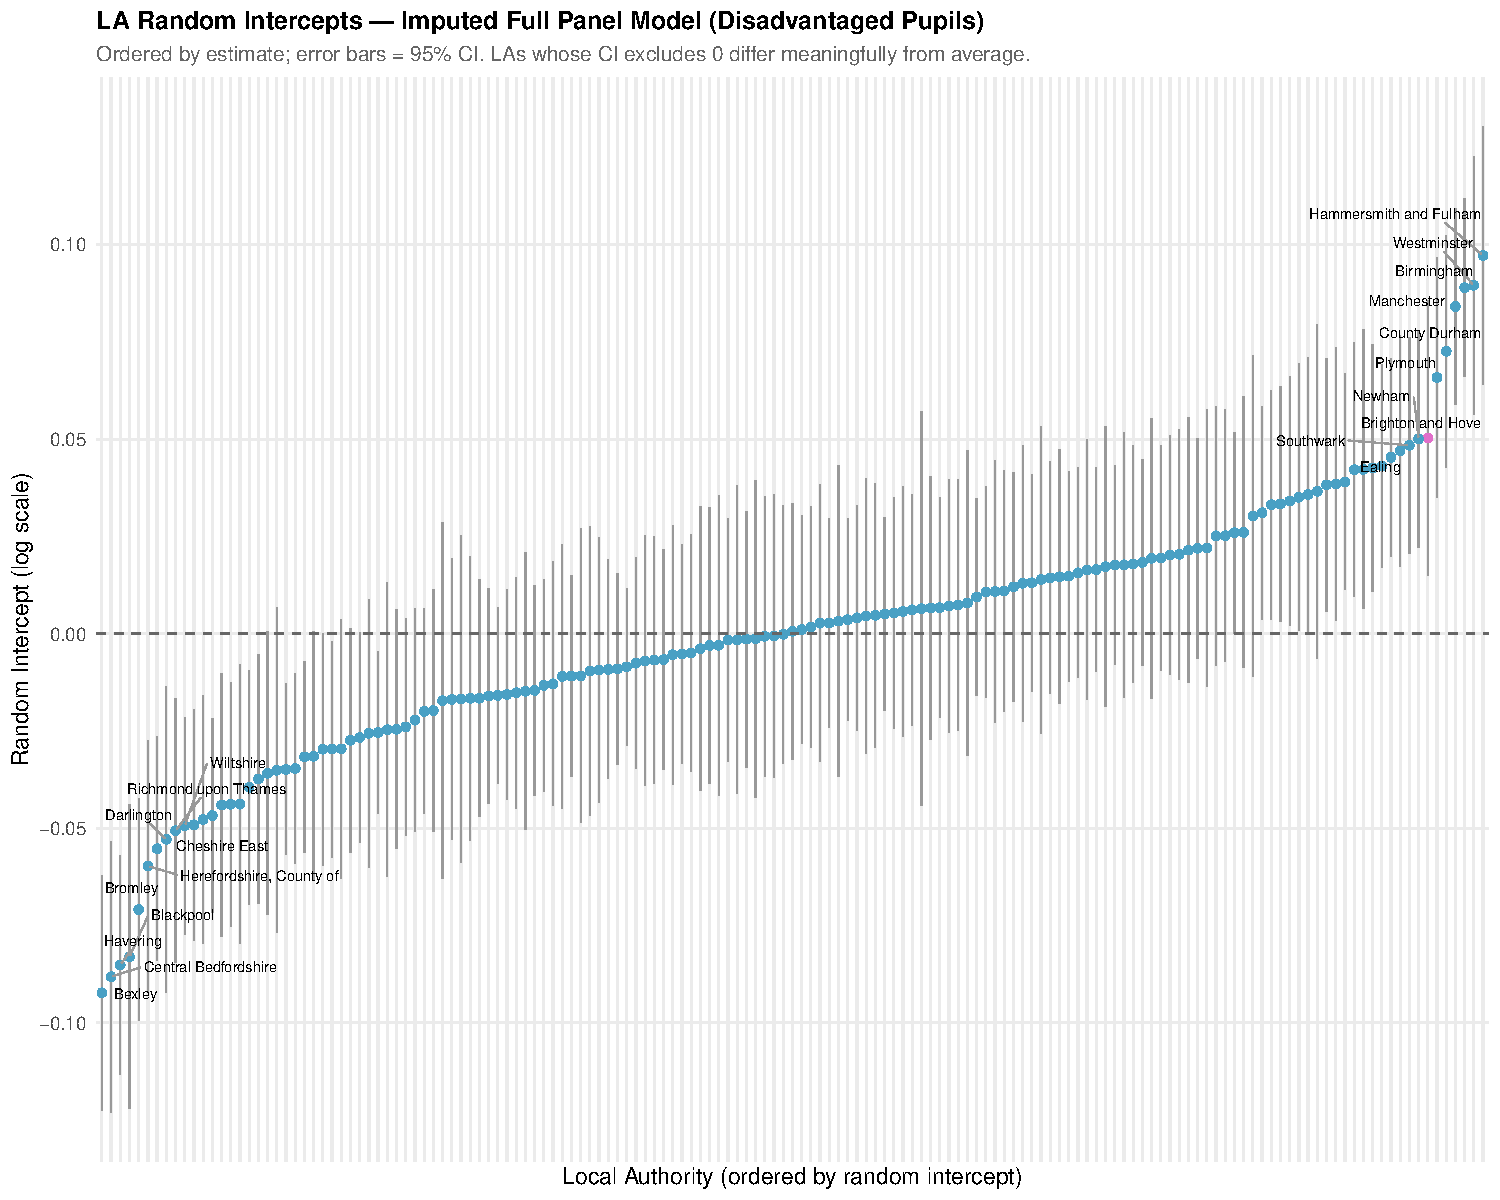
\includegraphics[keepaspectratio]{pulling_the_wrong_lever_files/figure-pdf/fig-caterpillar-1.pdf}}

}

\caption{\label{fig-caterpillar}Caterpillar plot of LA random intercepts
(imputed full panel model, Disadvantaged Pupils). Top and bottom 10 LAs
labelled; Brighton and Hove in pink.}

\end{figure}%

With this context, the policy starting point should have been somewhat
different to that experienced at the end of 2024. Rather than an
emergency needing radical changes to the secondary school system in the
city, we have a Local Education Authority that, given the structural
factors we know affect attainment, over-performing in the national
context --- in the top 10 LEAs for both disadvantaged and
non-disadvantaged attainment. Rather than what is the city doing wrong,
what is the city doing right? What are the factors (both within the gift
of the LEA to influence and not) not captured by the model that mean
that the city is over-performing? Are they home-based, such as parental
engagement? Is it something to do with school leadership and governance?
Local Authority services? School improvement programmes? These questions
will require additional data or qualitative follow-up to find the
answers to.

However, another question that follows that we can answer with the data
to hand is, what might be stopping the LEA effect from being even more
impressive? As large as it is for, say, Plymouth (another comparable
South Coast city) or larger cities like Manchester and Birmingham? What
might be the most effective policy levers to pull to improve overall
disadvantaged attainment even further in Brighton and Hove? And how do
the most effective levers compare with those that were chosen?

\subsection{Accelerating returns: comparing two candidate policy
levers}\label{accelerating-returns-comparing-two-candidate-policy-levers}

The national modelling in the last section established that the
relationships between attainment and most of its key school-level
predictors are non-linear. Because the model operates on log-transformed
variables, the same raw percentage-point change produces different
effects depending on where a school starts. Selecting FSM and absence
for illustration (as FSM levels were selected by the council as the main
policy lever through its redistribution policies, while absence stands
out from the national modelling) we can explore what this means. Reading
from right to left in Figure~\ref{fig-accelerating-returns} --- that is,
in the direction of policy improvement --- the returns to reducing both
absence and FSM \emph{accelerate} as schools improve. Each successive
percentage point of reduction buys a bigger predicted gain in Attainment
8 than the last.

But the two curves are not equal. Figure~\ref{fig-accelerating-returns}
places both variables on the same y-axis --- the predicted Attainment 8
gain from a 1 percentage point reduction --- allowing a direct
comparison of the two policy levers at every starting level.

\begin{figure}

\centering{

\pandocbounded{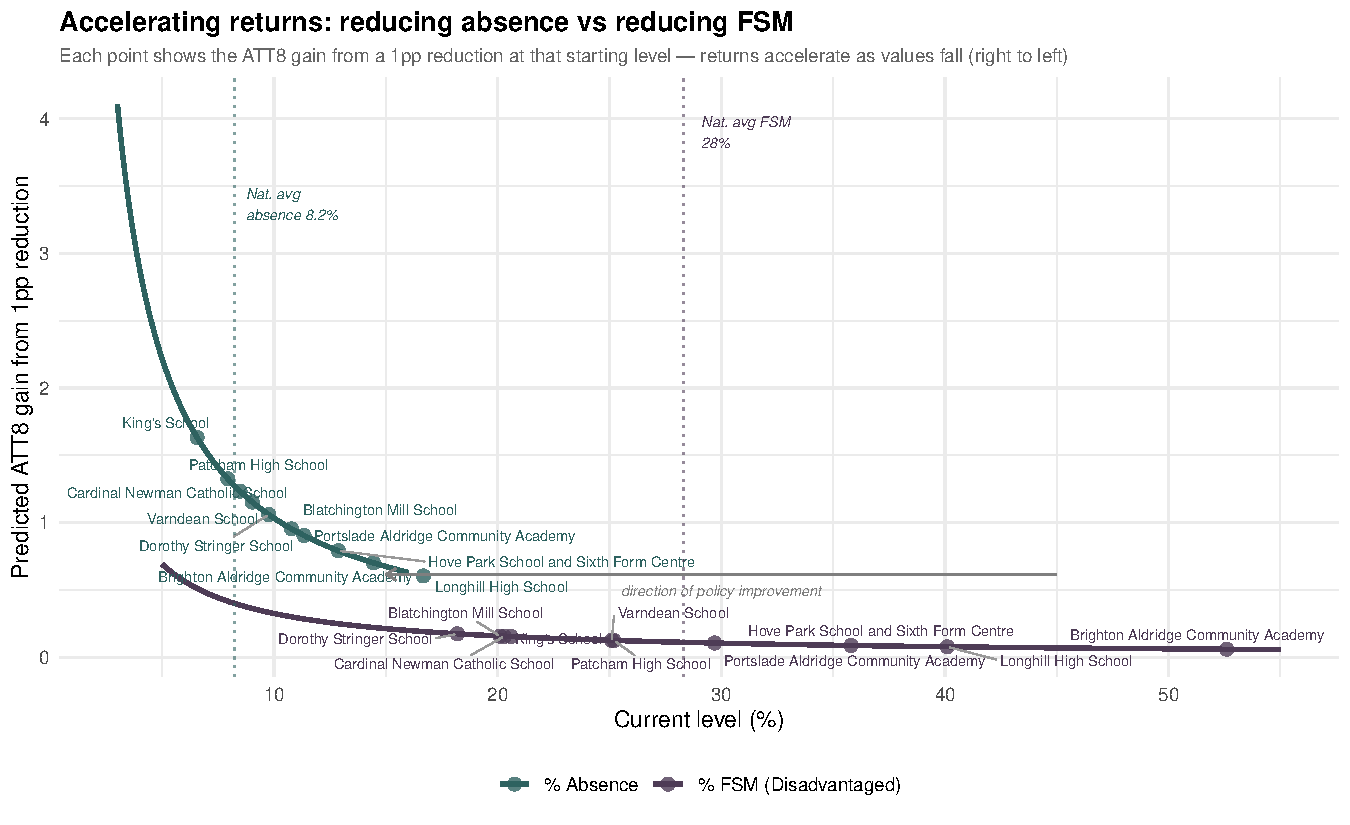
\includegraphics[keepaspectratio]{pulling_the_wrong_lever_files/figure-pdf/fig-accelerating-returns-1.pdf}}

}

\caption{\label{fig-accelerating-returns}Accelerating returns: each
percentage point of reduction buys a progressively larger ATT8 gain
(reading right to left). Absence (green) delivers substantially larger
gains than FSM (purple) at every level. Brighton \& Hove schools are
marked on each curve.}

\end{figure}%

Three things are immediately visible. First, the absence curve sits well
above the FSM curve at every starting level --- a 1 percentage point
reduction in absence always buys more predicted attainment than the same
reduction in FSM (although, of-course, these two cannot be compared
directly, but this is useful for illustrative purposes). Second, the gap
between the two curves \emph{widens} as values fall, meaning the
comparative advantage of targeting absence grows as schools improve.
Third, the Brighton \& Hove schools (marked on each curve) cluster in
the flatter right-hand portion for both variables, but the city's
position is far more extreme on absence than on FSM.

To put this in national context: Brighton \& Hove's mean school FSM rate
of 28.8\% is close to the national average of 28.3\%, placing the city
at roughly the 52nd percentile --- an unremarkable position. But the
city's mean absence rate of 10.8\% against a national average of 8.2\%
places it at the 99th percentile, 151st out of 152 local authorities ---
among the very worst in England. 8 out of 10 Brighton \& Hove secondary
schools have absence rates above the national school-level average.

When we standardise the x-axis so that both variables are measured in
standard deviations from their national means, the mismatch becomes even
starker. Figure~\ref{fig-accelerating-returns-standardised} shows that
Brighton \& Hove schools sit close to z = 0 for FSM (unremarkable) but
at z = +1 to +2 for absence (extreme national outliers). At the same
relative position in the national distribution, absence reduction
delivers substantially larger gains. When standardised by the Brighton
\& Hove spread of each variable, the absence coefficient is 2.6
times\footnote{derived by multiplying the model coefficient by the value
  of its log-transformed variable and then dividing one by the other} as
important as FSM for predicting attainment across the city's schools.

\begin{figure}

\centering{

\pandocbounded{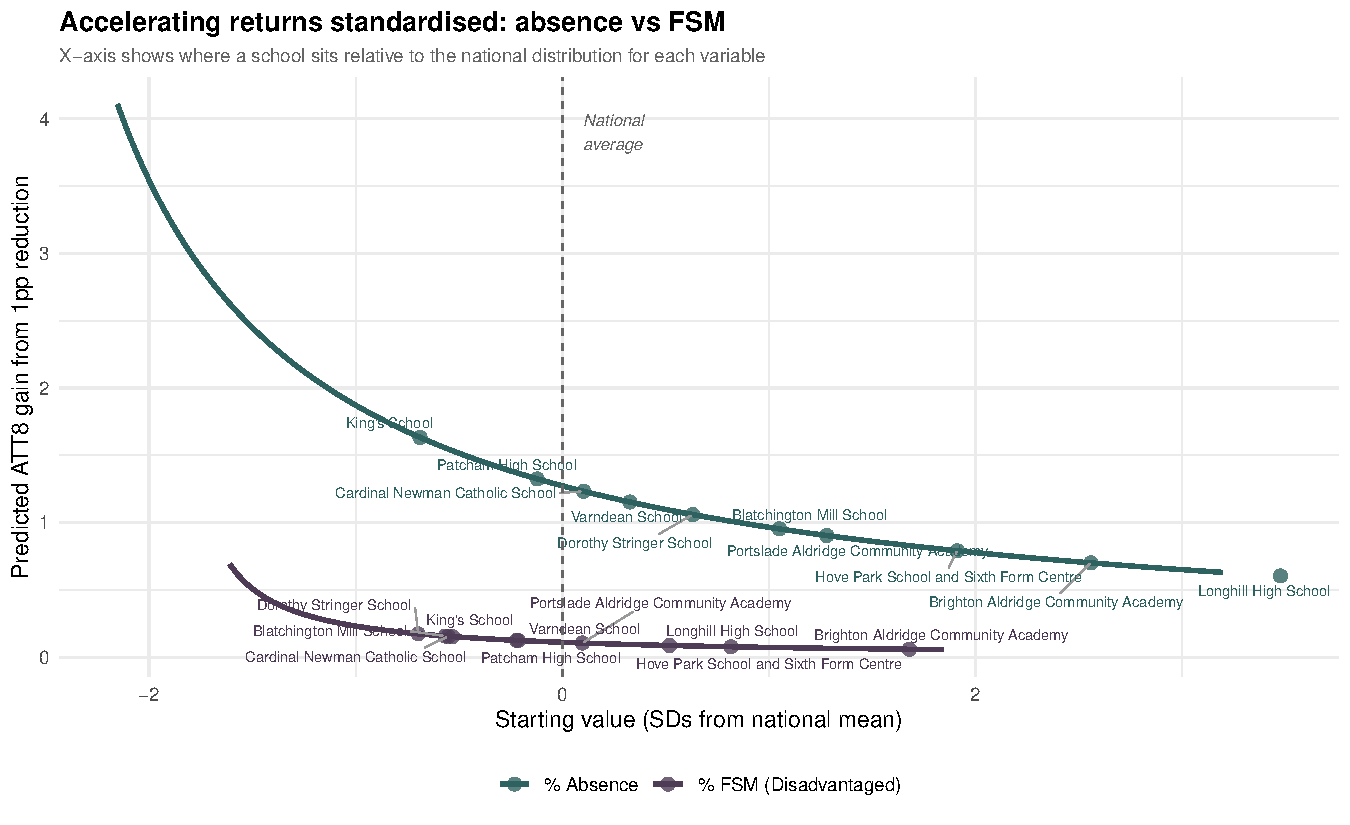
\includegraphics[keepaspectratio]{pulling_the_wrong_lever_files/figure-pdf/fig-accelerating-returns-standardised-1.pdf}}

}

\caption{\label{fig-accelerating-returns-standardised}Accelerating
returns standardised: x-axis shows SDs from the national mean. Brighton
\& Hove schools cluster near the national average for FSM but are
extreme outliers on absence.}

\end{figure}%

\subsubsection{Absence in Brighton and
Hove}\label{absence-in-brighton-and-hove}

Earlier analysis in this paper pointed to absence as being the most
important factor affecting attainment, but how do the absence levels in
Brighton and Hove compare to other LEAs in England?

\begin{table}

\caption{\label{tbl-absence}Highest-absence local authorities across all
panel years (mean school absence \%, rank).}

\centering{

\centering\begingroup\fontsize{10}{12}\selectfont

\begin{tabular}{l|r|r|r|r}
\hline
Local Authority & 2021-22 & 2022-23 & 2023-24 & 2024-25\\
\hline
Knowsley & 12.6\% (152/152) & 11.8\% (149/152) & 11.9\% (151/152) & 10.9\% (152/152)\\
\hline
\cellcolor[HTML]{fce4f1}{\textbf{Brighton and Hove}} & \cellcolor[HTML]{fce4f1}{\textbf{10.8\% (144/152)}} & \cellcolor[HTML]{fce4f1}{\textbf{10.5\% (137/152)}} & \cellcolor[HTML]{fce4f1}{\textbf{11.0\% (143/152)}} & \cellcolor[HTML]{fce4f1}{\textbf{10.8\% (151/152)}}\\
\hline
Newcastle upon Tyne & 12.2\% (151/152) & 12.9\% (152/152) & 11.4\% (150/152) & 10.6\% (150/152)\\
\hline
Southampton & 10.1\% (119/152) & 10.6\% (139/152) & 11.0\% (145/152) & 10.5\% (149/152)\\
\hline
Bradford & 11.5\% (149/152) & 11.9\% (150/152) & 11.2\% (147/152) & 10.3\% (148/152)\\
\hline
Plymouth & 11.1\% (147/152) & 10.8\% (144/152) & 11.3\% (149/152) & 10.2\% (147/152)\\
\hline
Middlesbrough & 11.8\% (150/152) & 12.9\% (151/152) & 12.2\% (152/152) & 10.1\% (146/152)\\
\hline
Sefton & 10.1\% (122/152) & 10.3\% (129/152) & 10.5\% (133/152) & 10.0\% (145/152)\\
\hline
Devon & 10.8\% (145/152) & 10.9\% (145/152) & 10.8\% (139/152) & 9.9\% (144/152)\\
\hline
Dorset & 10.3\% (134/152) & 10.2\% (127/152) & 10.7\% (137/152) & 9.9\% (143/152)\\
\hline
Halton & 10.1\% (118/152) & 10.3\% (131/152) & 11.0\% (144/152) & 9.8\% (142/152)\\
\hline
Blackpool & 9.8\% (103/152) & 11.1\% (147/152) & 11.3\% (148/152) & 9.8\% (141/152)\\
\hline
Hartlepool & 10.2\% (130/152) & 11.1\% (148/152) & 10.5\% (134/152) & 9.8\% (140/152)\\
\hline
Bristol, City of & 10.6\% (141/152) & 11.0\% (146/152) & 11.0\% (142/152) & 9.6\% (135/152)\\
\hline
Gateshead & 11.4\% (148/152) & 10.8\% (143/152) & 11.2\% (146/152) & 9.5\% (130/152)\\
\hline
St. Helens & 10.7\% (143/152) & 9.6\% (103/152) & 10.0\% (122/152) & 9.1\% (121/152)\\
\hline
Torbay & 10.9\% (146/152) & 10.2\% (125/152) & 10.3\% (126/152) & 8.2\% (75/152)\\
\hline
\end{tabular}
\endgroup{}

}

\end{table}%

As Table~\ref{tbl-absence} shows, Brighton and Hove had the 2nd worst
absence rate in England in 2024-25 --- it was in the top 10 in two of
the other three years where we have data. The direction of travel is, if
anything, deteriorating.

What would it mean if every Brighton \& Hove school brought its absence
rate down to the national school-level average of 8.2\%? A reasonable
ambition some may refer to as a policy ``no-brainer''?
Table~\ref{tbl-absence-national-avg-scenario} below shows the predicted
attainment gains\footnote{Note --- this table and the next use a
  simplified approximation of impact on Attainment 8. They take the
  model's coefficient for the variable of interest, compute the
  proportional change implied by a given shift on the log scale, and
  then multiply that proportional change by the city-wide mean observed
  Attainment 8 (or the school's own ATT8 where available) to convert it
  to Attainment 8 points. This is a shorthand for comparing schools
  side-by-side, but it produces slightly different point estimates from
  the full-model approach because it uses an average ATT8 as the base
  rather than each school's specific predicted score.}:

\begin{table}

\caption{\label{tbl-absence-national-avg-scenario}Potential Attainment
gains to be made at different schools in Brighton and Hove by moving
absence to the national average, 2024-25}

\centering{

\centering\begingroup\fontsize{10}{12}\selectfont

\begin{tabular}{l|r|r|r|r|r}
\hline
School & Current \% Absence & National Average (Target) & Reduction needed (pp) & Predicted ATT8 change (\%) & ≈ ATT8 points\\
\hline
Longhill High School & 16.7 & 8.2 & 8.4 & 16.25 & 5.3\\
\hline
Brighton Aldridge Community Academy & 14.4 & 8.2 & 6.2 & 12.74 & 4.6\\
\hline
Hove Park School and Sixth Form Centre & 12.9 & 8.2 & 4.6 & 10.01 & 4.1\\
\hline
Portslade Aldridge Community Academy & 11.3 & 8.2 & 3.1 & 7.07 & 3.0\\
\hline
Blatchington Mill School & 10.8 & 8.2 & 2.6 & 5.93 & 3.0\\
\hline
Dorothy Stringer School & 9.8 & 8.2 & 1.5 & 3.71 & 2.0\\
\hline
Varndean School & 9.0 & 8.2 & 0.8 & 1.98 & 1.0\\
\hline
Cardinal Newman Catholic School & 8.5 & 8.2 & 0.3 & 0.64 & 0.3\\
\hline
\end{tabular}
\endgroup{}

}

\end{table}%

8 out of 10 Brighton \& Hove schools currently have absence above the
national average. The potential gains for the schools with the highest
absence rates are substantial --- 3 to 5 GCSE points. Across these
schools, achieving the national average would produce predicted gains
averaging +2.9 Attainment 8 points per school. For disadvantaged pupils,
the gains would be even larger --- an average of +3.3 Attainment 8
points --- because the absence coefficient is larger for disadvantaged
pupils. Closing the absence gap to the national average would therefore
simultaneously raise overall attainment and narrow the disadvantage gap.

Brighton \& Hove's absence rates are not a necessary consequence of its
intake composition. The city has near-average levels of deprivation (FSM
rates at the national median) but near-worst absence. Many local
authorities with similar or higher FSM rates achieve substantially lower
absence. This suggests that the absence problem is driven by as-yet
unidentified local factors --- attendance culture and parental attitudes
towards attendance, enforcement practices, alternative provision use, or
community-level dynamics --- rather than being an unavoidable correlate
of disadvantage. As such it is, in principle, solvable, if the drivers
are properly identified.

The council has recently agreed to the creation cross-party working
group on schools and we would suggest this might be one of the most
pressing priorities for this group. It will certainly be the case that
within the broad-brush absence statistics, big differences in outcomes
might occur between, say, a few days missed for a family holiday by a
student who otherwise has an impeccable attendance record, a SEND
student who struggles with the school environment but who has strong
family support and a student with caring responsibilities who lives a
long way from their school and struggles to make the bus journeys
required for regular attendance. The city really needs to disaggregate
this attendance problem and devise strategies to deal with the different
causes in different ways.

\subsubsection{Concentrations of disadvantage in Brighton and
Hove}\label{concentrations-of-disadvantage-in-brighton-and-hove}

Given the council's policy focus in 2024 was on reducing concentrations
of disadvantage rather than on absence, it is worth quantifying what the
FSM lever can realistically deliver. The answer, as
Figure~\ref{fig-accelerating-returns} makes visually clear, is: far
less.

\begin{table}

\caption{\label{tbl-fsm-policy-scenario}Potential Attainment gains to be
made at different schools in Brighton and Hove by moving \%FSM to the
city average, 2024-25}

\centering{

\centering\begingroup\fontsize{10}{12}\selectfont

\begin{tabular}{l|r|r|r|r|r}
\hline
School & Current \% Absence & National Average (Target) & Reduction needed (pp) & Predicted ATT8 change (\%) & ≈ ATT8 points\\
\hline
Longhill High School & 16.7 & 8.2 & 8.4 & 16.25 & 5.3\\
\hline
Brighton Aldridge Community Academy & 14.4 & 8.2 & 6.2 & 12.74 & 4.6\\
\hline
Hove Park School and Sixth Form Centre & 12.9 & 8.2 & 4.6 & 10.01 & 4.1\\
\hline
Portslade Aldridge Community Academy & 11.3 & 8.2 & 3.1 & 7.07 & 3.0\\
\hline
Blatchington Mill School & 10.8 & 8.2 & 2.6 & 5.93 & 3.0\\
\hline
Dorothy Stringer School & 9.8 & 8.2 & 1.5 & 3.71 & 2.0\\
\hline
Varndean School & 9.0 & 8.2 & 0.8 & 1.98 & 1.0\\
\hline
Cardinal Newman Catholic School & 8.5 & 8.2 & 0.3 & 0.64 & 0.3\\
\hline
\end{tabular}
\endgroup{}

}

\end{table}%

Bringing the schools above the city average FSM rate down to it would
produce a predicted gain of roughly +0.9 GCSE points per school ---
modest gains that are dwarfed by the absence scenario above.

Table~\ref{tbl-fsm-policy-scenario} shows that for schools like BACA and
Longhill, even very dramatic reductions of 10-20\% in the proportion of
disadvantaged pupils would likely only bring relatively modest changes
to overall attainment at the school-level. And this is before factoring
in that the relationship for disadvantaged students, on average for
schools across England, works in the other direction. Of course, it
would never be as simple as reducing levels of absence having an
immediate and direct effect at the level predicted on attainment - these
modelled figures are indicative and don't account for a change in the
levels of one variable having an influence on the levels of another
(reducing absence, pushing up teacher sickness days, for example).
However they do allow us to make useful comparisons between actionable
policy levers relative to what we know about real situations in real
schools. We can say with more confidence that when comparing the impact
of reducing absence or disadvantage in a school, the absence coefficient
is roughly 2.6 times as important as disadvantage in predicting
attainment. This contradicts the council's assertion at the start of the
2024 consultation that results in the city are `driven by advantage': we
can say that this is not the case - if anything is depressing attainment
in the city's schools and `driving' results, given its impact and where
Brighton and Hove sits in the national league tables, it is absence.

\subsection{Brighton and Hove --- low prior
attainment}\label{brighton-and-hove-low-prior-attainment}

The examples above have zoomed in on the most important variable
(absence) and the one chosen by the council as their policy lever
(concentrations of disadvantage). However, as the earlier modelling
showed, there are other important factors to consider, the main one of
these being low prior attainment. The national modelling shows that
unless we control for the mediating effects of low prior attainment on
KS4 attainment, the effects of deprivation appear more damaging than
they are --- and indeed for schools with higher levels of deprived
students, all other things being equal, once low prior attainment is
accounted for, they are likely to achieve better results for their
deprived students than those with lower levels. In Brighton and Hove
schools, as shown in Figure~\ref{fig-prior-att}, the two are strongly
correlated, but without accounting for this factor, the FSM coefficient
absorbs both the direct deprivation effect and the indirect effect
operating through prior attainment.

\begin{figure}

\centering{

\pandocbounded{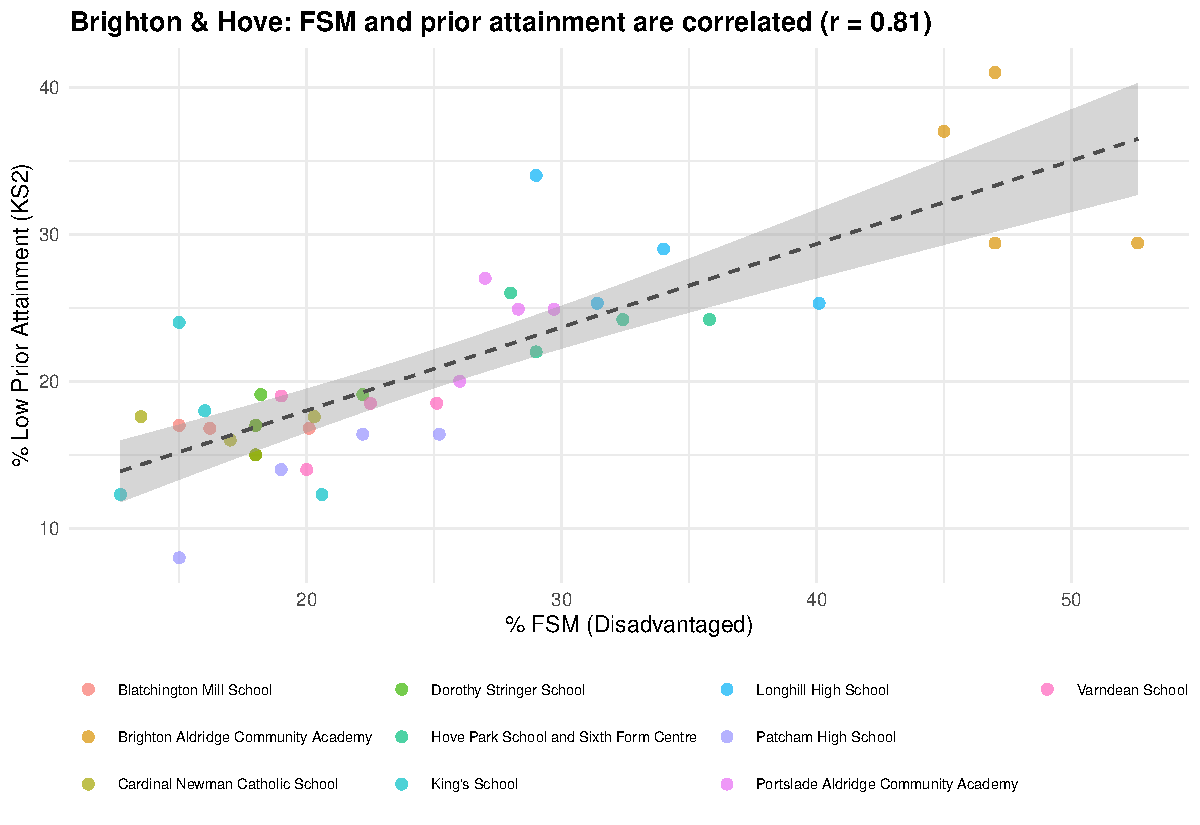
\includegraphics[keepaspectratio]{pulling_the_wrong_lever_files/figure-pdf/fig-prior-att-1.pdf}}

}

\caption{\label{fig-prior-att}Correlation between low prior attainment
and disadvantage across Brighton and Hove Schools, 2021-22 to 2024-25.}

\end{figure}%

\subsection{Alternative Local League
Tables}\label{alternative-local-league-tables}

One of the features of the debate in Brighton and Hove in 2024 related
to perceived school `quality' - and the desire for some to have choice
to send their children to schools thought to be better quality. For many
--- councillors and citizens alike --- impressions of secondary school
`quality' are predicated on Ofsted reports and raw GCSE results. Stories
in the local press ranking schools in the city according to just their
raw GCSE/Attainment 8 scores (Pring, 2025) certainly feed into a rather
reductive view of quality based on attainment that fails to account for
the varying intakes and cohorts across the schools in the city, both
inflating impressions of `quality' at some schools while unfairly
depressing it at others.

One advantage of the model-based national analysis presented is we can
compare what we observe with what the model says we should expect. The
models presented account for nearly all of the variation in Attainment 8
in schools across England over a 4-year period. Schools achieving scores
above those predicted are doing something (via factors we have not
measured --- perhaps related to behaviour management, governance,
culture and ethos) that means the average attainment of pupils in those
schools is better than expected. Conversely, schools with scores below
the model predictions are not achieving the attainment levels expected,
given their situation. Of course some of the residual variation could be
down to data limitations or deficiencies in variable selection, but in
modelling terms even if the data or variable selection are flawed in
some way, that so much variation is explained means our attention is
probably best focused on things we have not already covered in the
models to offer the best explanations for these residual values.

\begin{figure}

\centering{

\pandocbounded{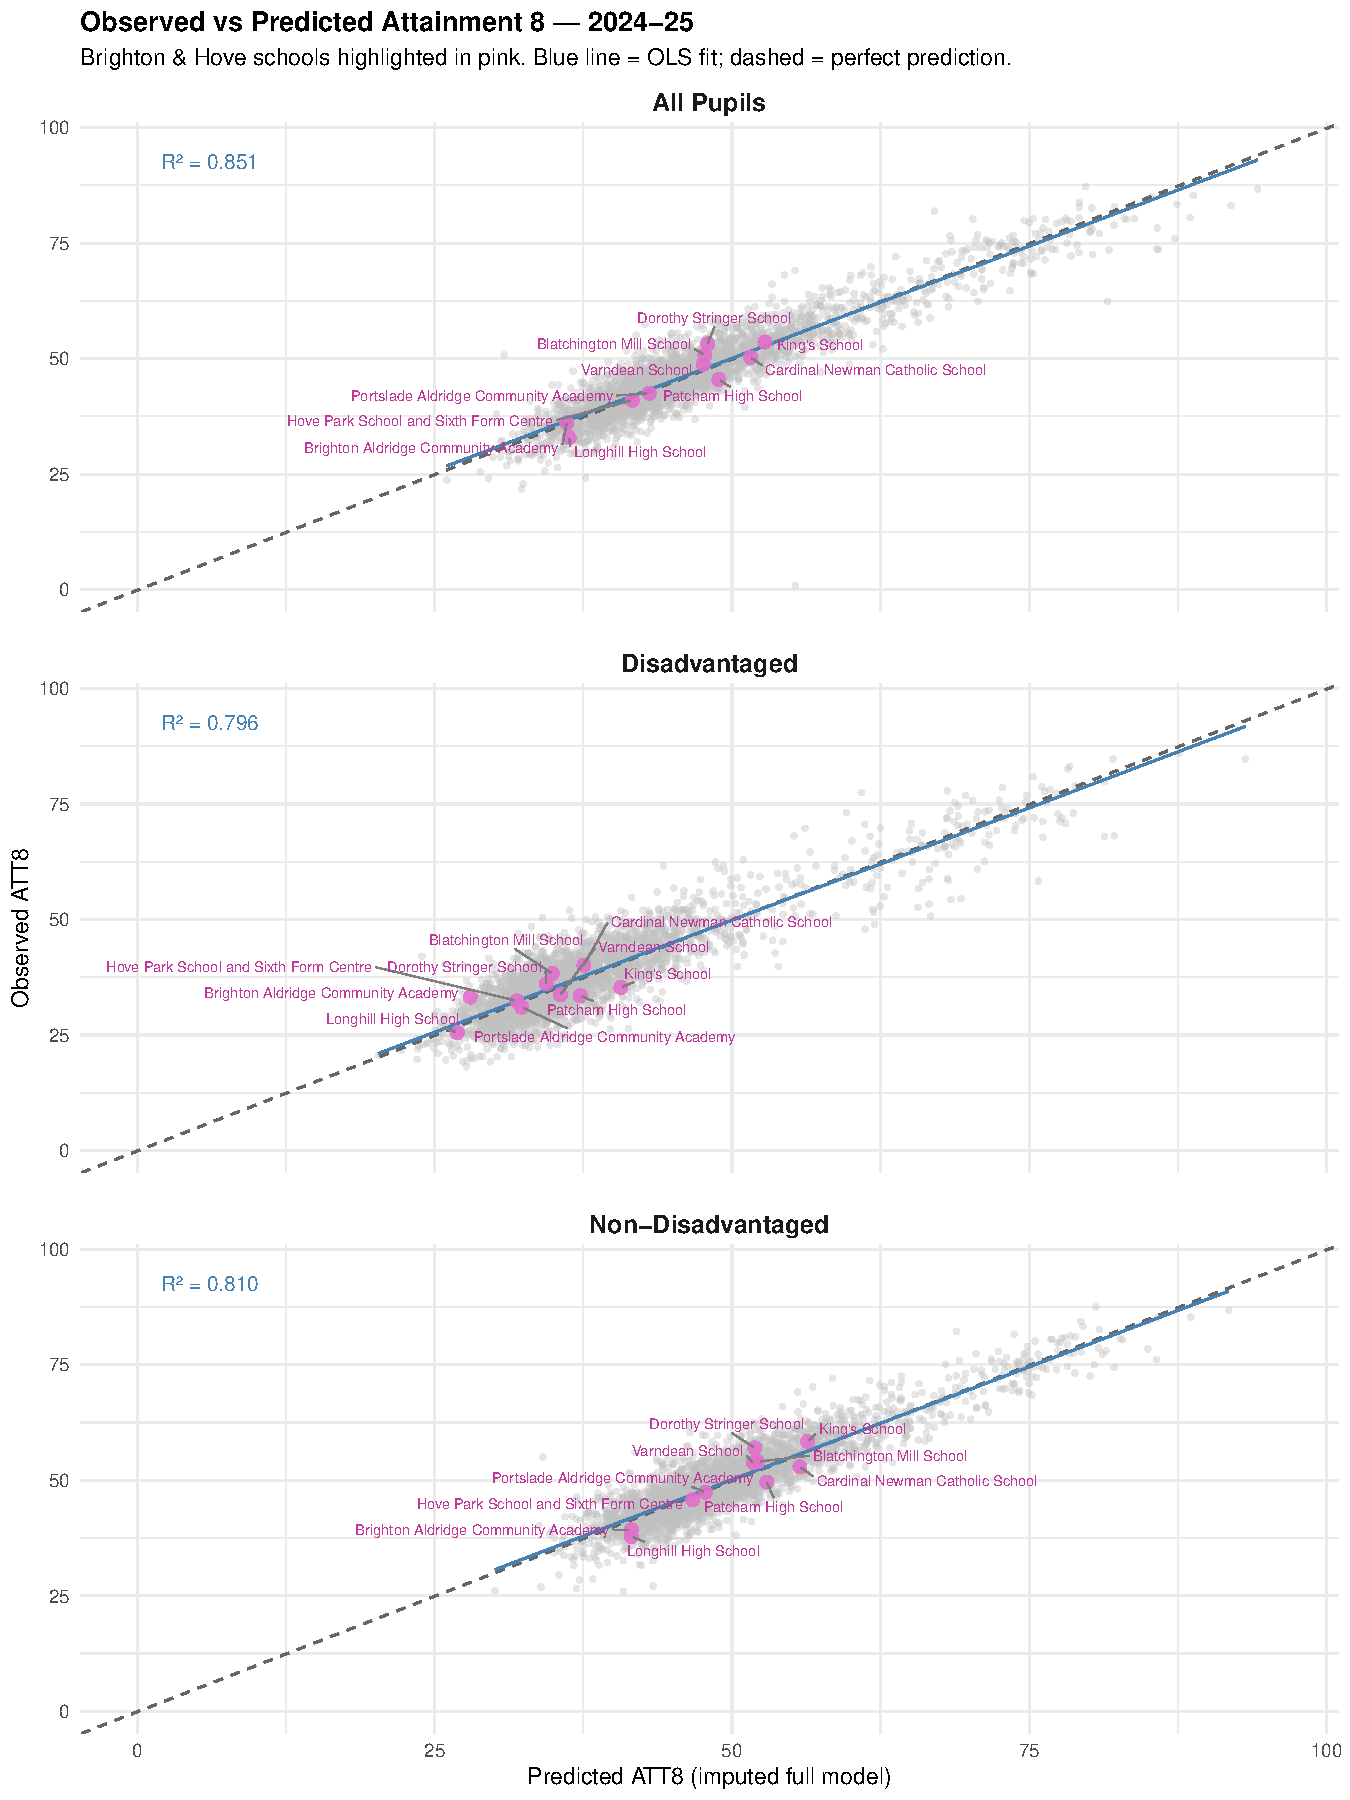
\includegraphics[keepaspectratio]{pulling_the_wrong_lever_files/figure-pdf/fig-obs-vs-pred-1.pdf}}

}

\caption{\label{fig-obs-vs-pred}Observed vs predicted Attainment 8 for
all schools (2024-25). Brighton \& Hove schools highlighted in pink and
labelled.}

\end{figure}%

Figure~\ref{fig-obs-vs-pred} is a visual representation of this. The
diagonal line represents where observed and predicted (by our model)
attainment match perfectly. The further vertically above or below the
line an individual school falls (in statistical terms, the greater its
residual), the better or worse it performs relative to expectations.
Brighton and Hove schools are highlighted and reveal an interesting
picture. Most schools are close to the attainment levels we would
expect, given their situations. Some perform much better than expected
--- e.g.~Dorothy Stringer School --- which achieves higher Attainment 8
results than expected for both disadvantaged and non-disadvantaged
pupils, whereas Longhill High School performs worse than expected on
both fronts.

The residuals in Figure~\ref{fig-obs-vs-pred} are captured in as set of
what we might term value-added league tables below in
Table~\ref{tbl-league-all} \& Table~\ref{tbl-league-dis}. Perhaps the
two most interesting schools in the city at other ends of this
alternative spectrum are Brighton Aldridge Community Academy (BACA) and
Patcham High School.

\begingroup\fontsize{10}{12}\selectfont

\begin{longtable}[t]{rlrrrr>{}r}

\caption{\label{tbl-league-all}}

\tabularnewline

\caption{}\\
\toprule
Rank & School & 2021-22 & 2022-23 & 2023-24 & 2024-25 & Mean Residual\\
\midrule
1 & Dorothy Stringer School & +3.5 & +3.8 & +2.8 & +5.2 & \cellcolor[HTML]{f5f5f5}{\textbf{+3.8}}\\
2 & Varndean School & +4.0 & +3.3 & +6.0 & +1.2 & \cellcolor[HTML]{f5f5f5}{\textbf{+3.6}}\\
3 & King's School & +4.8 & +0.1 & +5.9 & +0.8 & \cellcolor[HTML]{f5f5f5}{\textbf{+2.9}}\\
4 & Portslade Aldridge Community Academy & +2.9 & -0.4 & +3.1 & -0.5 & \cellcolor[HTML]{f5f5f5}{\textbf{+1.3}}\\
5 & Brighton Aldridge Community Academy & +2.0 & +1.2 & +0.4 & -0.0 & \cellcolor[HTML]{f5f5f5}{\textbf{+0.9}}\\
\addlinespace
6 & Blatchington Mill School & -2.2 & -0.8 & +2.5 & +3.1 & \cellcolor[HTML]{f5f5f5}{\textbf{+0.6}}\\
7 & Hove Park School and Sixth Form Centre & +0.6 & +2.0 & +0.4 & -0.6 & \cellcolor[HTML]{f5f5f5}{\textbf{+0.6}}\\
8 & Cardinal Newman Catholic School & +0.4 & -1.7 & +1.2 & -1.3 & \cellcolor[HTML]{f5f5f5}{\textbf{-0.3}}\\
9 & Longhill High School & +0.4 & -2.2 & -2.2 & -3.4 & \cellcolor[HTML]{f5f5f5}{\textbf{-1.8}}\\
10 & Patcham High School & -3.2 & -2.7 & -4.9 & -3.4 & \cellcolor[HTML]{f5f5f5}{\textbf{-3.6}}\\
\bottomrule

\end{longtable}

\endgroup{}

\begingroup\fontsize{10}{12}\selectfont

\begin{longtable}[t]{rlrrrr>{}r}

\caption{\label{tbl-league-dis}}

\tabularnewline

\caption{}\\
\toprule
Rank & School & 2021-22 & 2022-23 & 2023-24 & 2024-25 & Mean Residual\\
\midrule
1 & Brighton Aldridge Community Academy & +3.2 & -1.3 & +4.1 & +5.2 & \cellcolor[HTML]{f5f5f5}{\textbf{+2.8}}\\
2 & Varndean School & +3.2 & +3.6 & +4.5 & -1.9 & \cellcolor[HTML]{f5f5f5}{\textbf{+2.3}}\\
3 & Dorothy Stringer School & +2.9 & +3.2 & +0.3 & +1.7 & \cellcolor[HTML]{f5f5f5}{\textbf{+2.0}}\\
4 & Cardinal Newman Catholic School & +2.4 & -5.0 & +6.5 & +2.5 & \cellcolor[HTML]{f5f5f5}{\textbf{+1.6}}\\
5 & King's School & +5.8 & +0.9 & +4.4 & -5.4 & \cellcolor[HTML]{f5f5f5}{\textbf{+1.5}}\\
\addlinespace
6 & Blatchington Mill School & -5.4 & +1.3 & +5.2 & +3.4 & \cellcolor[HTML]{f5f5f5}{\textbf{+1.1}}\\
7 & Hove Park School and Sixth Form Centre & +2.4 & -1.7 & +1.3 & +0.5 & \cellcolor[HTML]{f5f5f5}{\textbf{+0.6}}\\
8 & Portslade Aldridge Community Academy & +2.6 & -4.0 & +4.7 & -1.3 & \cellcolor[HTML]{f5f5f5}{\textbf{+0.5}}\\
9 & Patcham High School & +3.8 & +1.6 & -11.9 & -3.7 & \cellcolor[HTML]{f5f5f5}{\textbf{-2.6}}\\
10 & Longhill High School & -4.6 & -6.2 & +0.8 & -1.4 & \cellcolor[HTML]{f5f5f5}{\textbf{-2.9}}\\
\bottomrule

\end{longtable}

\endgroup{}

The residuals are measured in raw GSCE point-score terms and show, on
average, how disadvantaged and non-disadvantaged pupils fare in
Attainment 8 terms, compared to other schools with similar profiles in
England and Wales. To re-iterate, this is not a raw-attainment table,
but an indication of the value-added (or taken away) by that school
compared to their peers in different LEAs, nationally.

BACA and Patcham are particularly interesting examples to zoom in on. In
the period of the 2024 consultation the public debate in the city
shifted slightly, away from how the council's proposals were going to
improve disadvantaged attainment to how they were facilitating parental
choice. Choice in this instance was largely to do with parents
perceiving their local options to be poor and wanting access to
alternatives. An activist group (Equity in Education\footnote{\url{https://educationequity.kit.com/}}
--- supported by another more established activist group --- Class
Divide\footnote{\url{https://www.classdivide.co.uk/}}) emerged from
within the BACA catchment advocating for parents to have more options
available to \emph{not} send their children to that school. At the time
BACAs Ofsted rating was `requires improvement' and its raw attainment
scores were some of the lowest in the city --- creating an impression of
that school being a poor option.

One of the outcomes that emerged from the vocal public debate, was a
considerable number of parents from the BACA catchment opting to send
their children to Patcham School (in the neighbouring catchment --- see
Figure~\ref{fig-catchments}) for entry in 2025 and 2026 --- a school
rated `Good' by Ofsted and with raw attainment scores placing somewhere
mid-table in the city. However, if we move beyond the raw attainment
scores and blunt single-word Ofsted ratings, a very different picture of
the two schools emerges. BACA is situated in one of the most
economically deprived parts of Brighton and Hove, Patcham, one of the
more economically prosperous. BACAs absence rates have been in excess of
the very high city average. Patcham is one of two schools in the City
with absence rates below the national average. The number of pupils
entitled to Free School Meals attending BACA is around 50\%, at Patcham
it is around 25\%. Around 30\% of the pupils attending BACA have low
prior attainment, at Patcham it is around 16\%. When we account for
these stark cohort differences in our model, a very different picture of
school effectiveness occurs.

As the league tables above reveal, in 2024-25, a disadvantaged pupil
attending BACA and taking their GSCEs would have, on average, left that
school with GCSEs 5-points higher than if they'd attended a similar
school with a similar profile elsewhere in England. Over the last 4
years, this would have averaged around 3 points higher. This is a boost
way in excess of the fraction of a point differences that might be
expected from altering the disadvantage mix in schools. BACA is doing
incredibly well for its disadvantaged students and indeed out-performs
every other school in the city by some margin --- even those which in
the popular imagination are viewed as the `best' or most desirable
schools in the city, e.g.~Varndean, Cardinal Newman. BACA in some ways
is the case study that illuminates the findings in the national data
earlier in this paper which showed that disadvantaged attainment is
higher in schools with bigger concentrations of disadvantaged students.
In April 2025, BACA received a new Ofsted report which rated it `Good'
in all 5 areas of provision\footnote{\url{https://reports.ofsted.gov.uk/provider/23/136164}}
--- a result unsurprising in the context of this data analysis, but
probably more surprising to anyone just looking at raw prior attainment
and previous Ofsted report.

If we contrast BACA --- the school popular narrative discouraged parents
from sending their children to --- with Patcham --- the school many from
BACA catchment in the end opted for, the differences on this alternative
league table are stark. Disadvantaged pupils attending Patcham on
average over the last 4 years and compared to other disadvantaged pupils
attending schools with similar profiles elsewhere in England, would
leave with around 2.6 GCSE points fewer than they might be expected to.
In 2023-24, the difference was in double figures. These differences have
been hidden from view amongst the comfortable mid-table position, in raw
attainment terms, the school has enjoyed. Now, of course, there might be
many reasons why parents would want to opt for Patcham High School over
BACA, but the nuance afforded to the effectiveness of these schools by
the modelling in this paper might have provided an alternative view that
could have made some of parents from BACA catchment who opted to send
their children to Patcham, make a different decision.

One thing other schools in the city certainly could learn from Patcham
High School is in how to improve attendance rates. The school is one of
only two in the city with attendance better than the national average.
This is an actionable policy lever at the school-level. Without a deeper
dive into attendance issues at the different schools in the city.
Indeed, given we now know where the real problems in Brighton and Hove
lie at the LEA level, one useful policy focus at the city level could
well be exploring how schools like Patcham are able to keep attendance
relatively high, while then allowing more school-level investigations
into where under-performance might be occurring given our new knowledge
of interacting structural drivers within the city.

\subsection{Brighton and Hove
Reflections}\label{brighton-and-hove-reflections}

\subsubsection{The Danger of Single-Lever Policy
Thinking}\label{the-danger-of-single-lever-policy-thinking}

The Brighton and Hove experience illustrates what can happen when policy
makers latch onto a single causal narrative and design interventions
around it to the exclusion of other --- potentially more impactful ---
factors. The council's 2024 proposals were built almost entirely on the
premise that attainment in the city was ``driven by economic advantage''
and that redistributing disadvantaged pupils more evenly across the
city's schools would narrow the attainment gap. The modelling presented
in this paper suggests this premise was, at best, incomplete and at
worst, fundamentally flawed.

As we have shown, concentrations of disadvantage are one of the weaker
levers available for influencing school-level Attainment 8 --- and for
disadvantaged pupils specifically, the direction of the effect runs
contrary to the assumptions underpinning the policy. Once absence and
low prior attainment are accounted for, the residual direct effect of
altering the social mix in schools is modest. As
Figure~\ref{fig-accelerating-returns} makes concrete: reducing absence
to the national average at the city's worst-affected schools could yield
gains of 3--5 GCSE points, whereas even dramatic reductions in
concentrations of disadvantage --- halving the FSM proportion at BACA,
for example --- would yield gains closer to 1--2 points, but crucially,
probably not for the disadvantaged pupils. The policy as designed was
pulling a lever with relatively little mechanical advantage while
ignoring one with considerably more.

This is not to say that concentrations of disadvantage are irrelevant
--- they are part of the story for all pupils and form part of the wider
ecology of school characteristics. But the political appeal of a social
mixing narrative --- with its apparently intuitive logic and its
socially progressive resonance --- in Brighton and Hove, crowded out a
more complex but more accurate understanding of the multiple,
interacting drivers of attainment. The result was a set of proposals
that risked disrupting a system that was, by national standards,
performing remarkably well for its disadvantaged students without a
clear evidential basis for expecting improvement.

We have also not touched upon the negative impacts of the policy that
was chosen. One of the main drivers of the huge opposition to the
proposals from within the city centred around the displacement outcome.
In order to affect more mixing in schools, beyond the mixing already
achieved by the 2023 Free School Meals priority, the 2024 consultation
proposed to reserve 20\% of places in central catchments for
out-of-catchment children ahead of in-catchment children, while reducing
the number of available places available in central catchment schools.
The net effect of this was, by the council's own calculations, that
significant numbers of children living in central catchments would be
unable to attend their catchment schools and be forced to attend another
outside of their catchment. In achieving greater mixing via these
policies, far more children would be having to travel much further to
school - either by opting-in or being forced out. As Thomson (2023)
showed in his analysis of NPD data, pupils who have to travel further to
school are absent more often. Therefore the notion that more mixing can
be achieved at ``almost no cost'' is false. If this extra travel
resulted in even slightly more absence from schools - then any
attainment gains would be undone immediately.

We should highlight that following widespread opposition and appeals to
the schools adjudicator, the proposed PAN reductions at central schools
were rejected and the 20\% out-of-catchment priority was reduced to 5\%.
This meant that following national offer day in March 2026, nearly all
in-catchment pupils who wanted to, were able to attend their catchment
school. However, while displacement was minimised, the full 5\%
out-of-catchment quota was taken up by opt-in students and significant
numbers of pupils were still opting to travel between schools in the
outer catchments where under-subscription allowed unhindered movement.
The single-lever policy reverberations are still being felt through the
choices expressed by parents.

\subsubsection{Absence: The Elephant in the
Room}\label{absence-the-elephant-in-the-room}

Perhaps the most striking finding from this analysis, in the Brighton
and Hove context, is the complete absence of absence from the policy
narrative in the period preceding the 2024 consultation and then again
with a more recent 2025 consultation. The city had the second worst
absence rate in England in 2024-25 and has been consistently among the
worst over the four years of our analysis. As the modelling
demonstrates, absence is by far the most powerful predictor of
school-level attainment, with its coefficient roughly 2.6 times larger
than that of disadvantage. For disadvantaged pupils, the effect is even
more pronounced --- nearly half of the variation in school-level
performance for this group is explained by whether pupils simply attend
classes.

The irony is considerable. Brighton and Hove ranks 7th best out of 152
LEAs for disadvantaged attainment after controlling for structural
factors --- the LEA random effect tells us that something about the
city's schools are delivering results well above what the national
picture would predict. Yet this strong underlying performance is being
dragged down by an absence problem that sits at the extreme end of the
national distribution. Were the city to bring its absence rates into
line with the national average, the potential attainment gains ---
particularly at schools like Longhill and BACA --- would dwarf anything
achievable through changes to the social composition of schools.

That the council chose to focus its policy energy on redistribution
rather than attendance is difficult to explain on evidential grounds.
Lobbying from the pressure group Class Divide, cannot be understated,
nor can the shift to a Labour majority in the council and accompanying
political motives. Other possibilities are that absence is a
fundamentally harder problem to solve than admissions policies --- more
diffuse in its causes, more resistant to top-down policy intervention,
and less amenable to the kind of structural reform that admissions
changes represent. But difficulty of implementation should not be
confused with importance of effect, and the failure to even acknowledge
absence as the primary drag on attainment in the city represents a
significant gap between the evidence and the policy response.

\subsubsection{The BACA Paradox}\label{the-baca-paradox}

The case of Brighton Aldridge Community Academy and the choices made by
parents in its catchment offers a particularly sharp illustration of the
damage that can be done when the public discourse around school quality
operates on crude metrics. During and after the 2024 consultation, a
vocal campaign emerged from the BACA catchment by the Equity in
Education group. It's difficult to ascertain whether this group emerged
\emph{because} of the choices already being made by parents who simply
wanted more options, or whether the campaign was the influencing factor
\emph{behind} parents looking for education options beyond their local
school --- possibly both. But data released as part of objections to the
Schools Adjudicator in the summer of 2025 revealed that a large number
of families from within the BACA catchment opted for Patcham High School
--- a school rated `Good' by Ofsted and sitting comfortably mid-table in
raw league tables. But at this time, all that most would have known
about BACA was it was a school with a `requires improvement' Ofsted
rating and raw attainment figures among the lowest in the city.

The alternative league table presented in this paper tells a very
different story. BACA is the best-performing school in the city for
disadvantaged pupils once we account for the structural factors that
shape its intake. In 2024-25, a disadvantaged pupil at BACA left with
GCSE results around 5 points higher than a comparable pupil at a similar
school elsewhere in England. Over the four-year period of analysis, the
average boost was around 3 points --- substantially higher than any
other school in the city, including those widely perceived as the `best'
options.

The implications are troubling. Parents, acting rationally on the basis
of the information available to them --- for example, raw league tables
and single-word Ofsted judgements as well as word-of-mouth and the
content and tone of public debates --- were actively choosing the
schools that might be a worse option if the value added by a school to
their child's likely GCSE outcomes were the most important factor.
BACA's April 2025 Ofsted upgrade to `Good' in all areas vindicates what
the data already showed, but came too late for the families who had
already made their decisions on the basis of incomplete and misleading
signals. This is not a criticism of those parents --- they were
operating in what we have described as a knowledge vacuum. It is,
however, a powerful argument for the kind of contextualised benchmarking
that this analysis makes possible.

\subsubsection{The Cost of Speed Over
Evidence}\label{the-cost-of-speed-over-evidence}

The institutional context in which these policy decisions were made
deserves reflection. The shift to a Leader and Cabinet system in May
2024 concentrated decision-making power and enabled policy to be enacted
through a whipped voting system without opposition amendments. The
consultation that followed in late 2024 was compressed in its timeline
and limited in its scope for genuine deliberative engagement. For those
of us on the receiving end of the proposals, the time available to
assemble, analyse and present counter-evidence was wholly inadequate for
the complexity of the issues at stake. It cannot be discounted that this
was an intended strategy by a council and its leadership keen to be seen
to be taking `bold', progressive action. They may have viewed time spent
putting a proposal with a small set of stakeholders, sufficient, but
policy without genuine critical scrutiny is destined to receive
push-back and runs the ultimate risk of failure and unintended
consequences.

This matters because the evidence base for secondary school attainment
is complex. As the literature review and modelling in this paper
demonstrate, the factors affecting outcomes are multiple, interacting,
non-linear, and context-dependent. Understanding why a particular policy
lever might or might not work in a specific local context requires more
than citing a single strand of academic work --- it requires the kind of
synthesis and contextualisation that takes time, analytical capacity,
and access to relevant data and tools. Institutional structures that
compress deliberation timelines are particularly dangerous when the
evidence requires careful handling and its implications
counterintuitive. Had the analysis presented here been available at the
outset --- or had the consultation process allowed time for it to be
developed --- the quality of public scrutiny would have been
substantially higher, even if the political outcome had ultimately
remained the same.

\subsubsection{What Is Driving the City's Over-Achievement? And What We
Don't Yet
Know}\label{what-is-driving-the-citys-over-achievement-and-what-we-dont-yet-know}

The LEA random effect for Brighton and Hove is large and statistically
significant across all three attainment groups. After accounting for the
structural factors in the model --- disadvantage, absence, prior
attainment, workforce characteristics, selectivity and segregation ---
schools in the city consistently outperform what the national picture
would predict. For disadvantaged pupils, the city ranks 7th; for
non-disadvantaged pupils, 5th; for all pupils, 4th in England.

This is a genuinely important finding that should re-frame the policy
conversation. The starting point for the 2024 consultation was a
narrative of failure --- the city was presented as uniquely failing its
disadvantaged students, sitting on a vast attainment gap, with radical
structural reform required to address the problem. The evidence suggests
the opposite: Brighton and Hove is one of the highest-performing LEAs in
the country once we account for the factors that we know drive
attainment. Rather than asking what the city is doing wrong, the more
productive question is what it is doing right --- and how that can be
protected and extended?

The honest answer is that we do not yet know what produces this LEA
effect. The random effect, by definition, captures variance that the
fixed-effect predictors do not explain. It could reflect high levels of
parental engagement and aspiration --- Brighton and Hove has a
well-educated population with a strong civic culture. It could relate to
the quality of school leadership and governance across the city, or to
effective local authority support services and school improvement
programmes. It could be something about the collaborative relationships
between schools, or community factors that are difficult to quantify.
Identifying the sources of this over-performance is an important
research question in its own right, and one that could require
additional qualitative investigation or access to pupil-level data that
goes beyond what is publicly available. What is clear, however, is that
policy interventions which risk disrupting a well-functioning system
without understanding what makes it function well carry substantial
downside risk.

\subsubsection{Conflicting Incentives: Viability Versus
Attainment}\label{conflicting-incentives-viability-versus-attainment}

It is worth acknowledging directly what was only partially articulated
during the consultation: that a significant driver of the council's
proposals was financial rather than educational. The attempts to reduce
Published Admission Numbers (rejected in the end after appeal to the
Schools Adjudicator by parents and schools alike) at popular central
schools and the creation of out-of-catchment priority places were
designed, at least in part, to redirect pupil flows toward
under-subscribed schools on the geographic periphery of the city.
Keeping schools with declining numbers financially viable is a
legitimate concern for any local education authority managing a school
estate.

However, there is an inherent tension between optimising for financial
sustainability and optimising for educational outcomes. If the net
effect of these pupil flows is to move children from schools that are
adding more value (in the contextualised sense demonstrated in this
paper) to schools that are adding less, the aggregate impact on
city-wide attainment could be negative. And if a school is forced to
close because of poor strategic planning --- parents not wanting to send
their children miles out of town when there are more desirable and
closer schools --- is not the fault of the parents, but a failure of
policy makers to listen, acknowledge this reality, and come up with
alternative designs. Furthermore, the longer journeys that both `opt-in'
out-of-catchment priority and `forced-out' in-catchment pupils further
down the priority list would face, carry their own risks. As Thomson
(2023) has documented, journey length and complexity are associated with
higher absence rates --- and given that absence is already the city's
most acute problem and the strongest predictor of attainment, a policy
that even marginally increases absence for some pupils could be
counterproductive in attainment terms. The financial case for the
proposals and the educational case needed to be weighed against each
other transparently, and it is not clear that this trade-off was
adequately acknowledged during the public consultation periods.

\subsubsection{Lessons for Other Local Education
Authorities}\label{lessons-for-other-local-education-authorities}

Brighton and Hove's experience carries implications well beyond the
city. The new DfE (2026) white paper sets national ambitions to halve
the disadvantage attainment gap, improve attendance, reform admissions
and tackle place-based disadvantage --- including in coastal towns
likely to be targeted by the new ``Mission Coastal'' initiative.
Brighton and Hove may well be one such target.

The lesson from this case study is that national ambitions, however
laudable, will founder if they are pursued at the local level without
adequate analytical infrastructure. Every LEA has a different profile of
challenges --- different positions along the non-linear curves that
relate disadvantage, absence, prior attainment and other factors, to
outcomes. What works in one context may be irrelevant or
counterproductive in another --- cities, towns or collections of smaller
settlements within LEAs with different configurations of schools, social
geographies and education profiles. The open data published by the
Department for Education provides most of the raw materials needed to
understand these local contexts, but as we have argued throughout this
paper, there is a crucial gap between the availability of raw data and
the availability of actionable, contextualised intelligence that is
accessible to the people who need it --- councillors, school leaders,
governors, and parents responding to statutory consultations.

We hope that the analysis we have presented and the tool we are about to
introduce go some way towards bridging that gap. But we also recognise
that tools alone are insufficient. What is also required is a culture of
evidence-informed policy making that resists the temptation to reach for
simple narratives, that takes seriously the complexity and
context-dependence of educational outcomes, and that creates
institutional space for genuine deliberation before irreversible
decisions are made. Brighton and Hove's experience should serve as a
cautionary tale --- but also, given the underlying strength of its
schools, as a reminder of what is possible when the focus shifts from
what is going wrong to understanding and building on what is going
right.

\section{The School Attainment Policy
Simulator}\label{the-school-attainment-policy-simulator}

\subsection{Development Workflow}\label{development-workflow}

The analysis we have presented here has necessarily zoomed in on our
case study city to illustrate the issues. But we cannot hope to foster
an enhanced collective intelligence across LEAs and within and between
communities when insights are hidden within mountains of available but
largely unprocessed, tabular data. Part of this work has been funded by
the UKRI National AI Research Hub for Collective Intelligence ---
AI4CI\footnote{\url{https://ai4ci.ac.uk/about-the-hub/}} --- an
initiative to explore how emerging Artificial Intelligence tools can be
brought to bear to help advance our collective intelligence across a
range of domains including city planning and urban intelligence.

To this end, we have leant on the capabilities of Anthropic's Claude
Opus 4.6\footnote{\url{https://www.anthropic.com/claude/opus}} to assist
in firstly, scaling up the initial analysis developed by one of us since
the initial 2024 consultation --- much of it available
\href{https://adamdennett.github.io/BH_Schools_Consultation/about.html}{here}\footnote{\url{https://adamdennett.github.io/BH_Schools_Consultation/about.html}}
and via teaching materials developed by one of us as part of the
CASA0007 Quantitative Methods MSc module, available
\href{https://huanfachen.github.io/QM/}{here}\footnote{\url{https://huanfachen.github.io/QM/}},
and then secondly building this into an interactive tool. The
exploratory descriptive analyses and explanatory models were developed
without the assistance of Claude, however the data processing, cleaning,
panel creation and scaling up of the analysis, implementing these models
across multiple years and many iterations, could not have been achieved
within the timeframes we have been able to achieve without this
assistance. The Policy Simulator Tool is built in R Shiny\footnote{\url{https://shiny.posit.co/}}
and takes these foundational analyses and makes them both interactive
and dynamic. Most of this front-end development was facilitated by
Claude Opus 4.6 under iterative instruction.

\subsection{The Attainment Policy Simulator
Tool}\label{the-attainment-policy-simulator-tool}

The tool can be accessed here ---
\url{https://adam-dennett.shinyapps.io/School_Attainment_Policy_Simulator/}
--- the tool is built on all of the open DfE data we have already
described in the earlier analysis in this paper and in the supplementary
materials linked to --- mainly the last 4-years of attainment and other
school-level statistics. It contains exactly the same underlying
multilevel linear mixed effects model as has been described. The front
page --- Figure~\ref{fig-simulator-front} --- introduces the tool and
its functionality in more detail and is the gateway to analytical tabs,
detailed in Table~\ref{tbl-simulator-tabs}.

\begin{figure}

\centering{

\pandocbounded{\includegraphics[keepaspectratio]{output/figures/policy_sim.png}}

}

\caption{\label{fig-simulator-front}Front Page of the Policy Simulator
Tool.}

\end{figure}%

\begingroup\fontsize{11}{13}\selectfont

\begin{longtable}[t]{>{\raggedright\arraybackslash}p{10em}>{\raggedright\arraybackslash}p{40em}}

\caption{\label{tbl-simulator-tabs}Analysis Tabs Available in the Policy
Simulator.}

\tabularnewline

\toprule
Tab & What it does\\
\midrule
\textbf{School Finder} & Search for a school by name or Local Authority. View it on a map, see key statistics, and send it to the Policy Simulator for deeper analysis.\\
\textbf{Find My Twin} & Select a school and find its 'twin' — another school with the most similar contextual characteristics (pupil intake, absence, workforce, school type). Attainment outcomes are shown for comparison but excluded from the matching.\\
\textbf{Observed vs Predicted} & An interactive scatter plot comparing every school's actual attainment against its model-predicted value. Schools above the line are outperforming; those below are underperforming relative to expectations.\\
\textbf{Policy Simulator} & The core tool. Adjust school-level variables — absence rates, pupil composition, teacher retention, leadership pay, and more — to see the predicted impact on attainment. Crucially, some of these relationships are non-linear, so the simulator reveals where small changes matter most and where returns diminish.\\
\textbf{LA Overview} & A Local Authority-level view showing how schools within an LA perform relative to expectations, with a distribution chart comparing the LA against the national picture.\\
\addlinespace
\textbf{LA Typology} & A data-driven classification of Local Authorities into clusters based on over 200 indicators. Explore which LAs face similar challenges and compare their profiles on an interactive map.\\
\textbf{Cluster Analysis} & Radar charts and summary statistics for each LA cluster, making it easy to compare groups and identify shared characteristics.\\
\textbf{Model Info} & Technical detail: model coefficients, fit statistics, diagnostics, and caveats. Useful for understanding the model's strengths and limitations.\\
\bottomrule

\end{longtable}

\endgroup{}

The tool allows for the easy visualisation of descriptive raw and
modelled statistics at both the local authority and school levels.
Perhaps most usefully for school leaders and policy makers, the
simulator tab allows users to select a school and using the coefficients
and linear or log-linear associations with the predictors used in the
model, adjust sliders to see how changes in these variables might impact
the attainment of all pupils, disadvantaged and non-disadvantaged
pupils, at the school level.

\begin{figure}

\centering{

\pandocbounded{\includegraphics[keepaspectratio]{output/figures/policy_sim_sliders.png}}

}

\caption{\label{fig-simulator-sliders}Screenshot of the Dynamic Elements
of the Policy Simulator.}

\end{figure}%

The simulator is not designed to give definitive school level
predictions --- this is not its intended purpose and the sliders when
moved will not and cannot account for potential changes in the
coefficient values or levels associated with other variables in a truly
inter-connected way. However, what it can do is zoom in on the unique
starting position of any school in the dataset and allow users to see
what the most important variable influencing attainment might be at that
school and, potentially, what the most impactful lever could be.

This tool is far from the finished article, but it shows how the volumes
of openly published DfE data can be used to provide more intuitive
insights into the issues and challenges faced by different schools and
different local authorities --- providing much needed local context in
debates which, as our experience in Brighton and Hove has shown, are
often not as well informed by up-to date, geographically specific and
timely data as they could be.

\section{Conclusions}\label{conclusions}

This paper set out to demonstrate that the Department for Education's
open data publications are a substantially underutilised resource for
understanding and improving secondary school attainment in England. We
believe the analysis and the tool presented here make that case
convincingly. School-level attainment is remarkably predictable from a
small number of readily available variables, and that predictability ---
once harnessed --- creates an opportunity for far better-informed local
policy making than was evident in our case study city.

We should be clear about what this analysis can and cannot claim. These
are school-level models built from aggregate published data, not
pupil-level analyses. The associations we identify are not experimental
estimates of causal effects --- they are the best approximations
available from observational data structured to account for confounding
and mediation across a rich set of predictors and hierarchical grouping
factors. The Policy Simulator tool translates these associations into
indicative, not definitive, projections. We do not claim that reducing
absence by a given number of percentage points will mechanically produce
the predicted gain in Attainment 8 --- the real world is more complex
than any model can capture. What we do claim is that these models are
accurate enough, and the patterns consistent enough across years and
specifications, to substantially improve the quality of the conversation
around what matters most for school attainment and where policy effort
is best directed.

We are yet to see the outcome of some follow-up work that the council
has commissioned to explore the effectiveness of their Free School Meal
priority policy, however the evidence from the four years of analysis in
this work is that, at the school level at least, we would not expect big
improvements in attainment from changes to the social composition of
schools.

The School Attainment Policy Simulator developed as part of this work
represents an attempt to bridge the gap between available open data and
the actionable, contextualised intelligence that the people making
decisions actually need. We do not claim it is the finished article ---
it can and should be refined, extended and subjected to critical
scrutiny. But we believe it demonstrates what is possible when open data
is combined with appropriate analytical methods and made accessible
through interactive tools. Its development was substantially accelerated
by the use of large language model assistance --- specifically
Anthropic's Claude --- as part of work funded by the UKRI AI4CI hub, and
stands as an example of how emerging AI capabilities can enhance
collective intelligence around complex policy questions, especially
where capacity is low. We should make clear that expert interaction and
iteration was crucial throughout --- this was not an experience of
`letting an AI do it all' but more akin to working with a highly skilled
junior front-end developer who, while technically adept, needed careful
guidance around architecture and scrutiny of outputs along the way.

Our recommendations are directed at three audiences. For the Department
for Education, we would urge continued investment in the quality and
timeliness of open data publications, and consideration of how the
analytical infrastructure demonstrated here might be supported or
replicated at scale --- perhaps through funding for local authority
analytical capacity or the development of nationally maintained
benchmarking tools that go beyond raw league tables. For local education
authorities, the lesson from Brighton and Hove is that evidence-informed
policy requires more than good intentions and a single strand of
academic literature --- it demands a willingness to engage with
complexity, to resist the allure of simple narratives, and to create
institutional space for genuine deliberation before decisions are made.
For schools, governing bodies and parents, we hope this work
demonstrates that there is more to school quality than raw Attainment 8
scores and single-word Ofsted ratings --- and that contextualised
benchmarking of the kind presented here offers a fairer and more useful
basis for understanding how well a school is serving its pupils.

Our case study of Brighton and Hove --- motivated by experiences of the
2024 and 2025 public consultations, should serve as both a cautionary
tale and a source of encouragement. The caution is that policy made in
haste, anchored to a single causal narrative and implemented without
adequate regard for the full range of evidence, risks doing more harm
than good --- particularly when it could disrupt a system that is, by
most measures, working well. The encouragement is that the raw materials
for better policy already exist in the open data the Department for
Education publishes, and that with the right analytical tools and a
commitment to evidence over ideology, it is possible to understand with
considerable precision what drives attainment in any local context and
where the most productive interventions lie. The challenge now is to
ensure that this understanding reaches the people who need it, in a form
they can use, before the decisions are made --- not after.

\section*{References}\label{references}
\addcontentsline{toc}{section}{References}

\phantomsection\label{refs}
\begin{CSLReferences}{1}{1}
\bibitem[\citeproctext]{ref-Allen2018}
Allen R, Burgess S and Mayo J (2018) The teacher labour market, teacher
turnover and disadvantaged schools: New evidence for {England}.
\emph{Education Economics} 26(1): 4--23. DOI:
\href{https://doi.org/10.1080/09645292.2017.1366425}{10.1080/09645292.2017.1366425}.

\bibitem[\citeproctext]{ref-Allen2013}
Allen R, Burgess S and McKenna L (2013) The short-run impact of using
lotteries for school admissions: Early results from {Brighton} and
{Hove}'s reforms. \emph{Transactions of the Institute of British
Geographers} 38(1): 149--166. DOI:
\href{https://doi.org/10.1111/j.1475-5661.2012.00511.x}{10.1111/j.1475-5661.2012.00511.x}.

\bibitem[\citeproctext]{ref-AllenSims2018}
Allen R and Sims S (2018) Do pupils from low-income families get
low-quality teachers? {Indirect} evidence from {English} schools.
\emph{Oxford Review of Education} 44(4): 441--458. DOI:
\href{https://doi.org/10.1080/03054985.2017.1421152}{10.1080/03054985.2017.1421152}.

\bibitem[\citeproctext]{ref-AllenWest2011}
Allen R and West A (2011) Why do faith secondary schools have advantaged
intakes? {The} relative importance of neighbourhood characteristics,
social background and religious identification amongst parents.
\emph{British Educational Research Journal} 37(4): 691--712. DOI:
\href{https://doi.org/10.1080/01411926.2010.489145}{10.1080/01411926.2010.489145}.

\bibitem[\citeproctext]{ref-Anders2024}
Anders J, Green F, Henderson M, et al. (2024) Private school pupils'
performance in {GCSEs} (and {IGCSEs}). \emph{Cambridge Journal of
Education} 54(6): 795--813. DOI:
\href{https://doi.org/10.1080/0305764X.2024.2420611}{10.1080/0305764X.2024.2420611}.

\bibitem[\citeproctext]{ref-AndrewsJohnes2016}
Andrews J and Johnes R (2016)
\emph{\href{https://dera.ioe.ac.uk/id/eprint/27949/1/Pupil_characteristics_and_performance_at_faith_schools.pdf}{Faith
{Schools}, pupil performance, and social selection}}. Education Policy
Institute.

\bibitem[\citeproctext]{ref-Bernhard2024}
Bernhard R, McDermott T, Hasenhüttl C, et al. (2024) A focus on quality
of teaching in schools increases students' progress of attainment.
{Evidence} from {English} secondary schools. \emph{School Effectiveness
and School Improvement} 35(4): 506--530. DOI:
\href{https://doi.org/10.1080/09243453.2024.2398601}{10.1080/09243453.2024.2398601}.

\bibitem[\citeproctext]{ref-Burgess2018}
Burgess S, Crawford C and Macmillan L (2018) Access to grammar schools
by socio-economic status. \emph{Environment and Planning A: Economy and
Space} 50(7): 1381--1385. DOI:
\href{https://doi.org/10.1177/0308518X18787820}{10.1177/0308518X18787820}.

\bibitem[\citeproctext]{ref-Burgess2022}
Burgess S, Rawal S and Taylor E (2022)
\emph{\href{https://www.nuffieldfoundation.org/project/characterising-effective-teaching-2}{Characterising
effective teaching}}. Nuffield Foundation.

\bibitem[\citeproctext]{ref-Burgess2023}
Burgess S, Rawal S and Taylor ES (2023) Teachers' use of class time and
student achievement. \emph{Economics of Education Review} 94: 102405.
DOI:
\href{https://doi.org/10.1016/j.econedurev.2023.102405}{10.1016/j.econedurev.2023.102405}.

\bibitem[\citeproctext]{ref-Chazan2000}
Chazan M (2000) Social {Disadvantage} and {Disruptive} {Behaviour} in
{School}. In: \emph{Combating {Educational} {Disadvantage}}. Routledge.

\bibitem[\citeproctext]{ref-SocialMobilityCommission2021}
Commission SM (2021)
\href{https://www.gov.uk/government/news/smc-responds-to-report-on-white-working-class-pupils-being-let-down}{The
{Social} {Mobility} {Commission} ({SMC}) responds to report on {White}
working class pupils being {`let down'}}. \emph{GOV.UK}.

\bibitem[\citeproctext]{ref-HouseofCommons2021}
Commons Education Committee H of (2021)
\href{https://committees.parliament.uk/committee/203/education-committee/news/156024/forgotten-white-workingclass-pupils-let-down-by-decades-of-neglect-mps-say/}{{`{Forgotten}'}
{White} working-class pupils let down by decades of neglect, {MPs} say -
{Committees} - {UK} {Parliament}}.

\bibitem[\citeproctext]{ref-DfE2022}
DfE (2022)
\href{https://explore-education-statistics.service.gov.uk/find-statistics/the-link-between-absence-and-attainment-at-ks2-and-ks4/2018-19}{The
link between absence and attainment at {KS2} and {KS4}, {Academic} year
2018/19}.

\bibitem[\citeproctext]{ref-DfE2024}
DfE (2024)
\href{https://www.gov.uk/government/publications/working-together-to-improve-school-attendance}{Working
together to improve school attendance}. \emph{GOV.UK}.

\bibitem[\citeproctext]{ref-DfE2025a}
DfE (2025a)
\emph{\href{https://www.gov.uk/government/publications/link-between-attendance-and-attainment}{Link
between attendance and attainment}}. London: Department for Education.

\bibitem[\citeproctext]{ref-DfE2025b}
DfE (2025b)
\href{https://explore-education-statistics.service.gov.uk/find-statistics/pupil-absence-in-schools-in-england/2024-25-autumn-and-spring-term}{Pupil
absence in schools in {England}, {Autumn} and spring term 2024/25}.

\bibitem[\citeproctext]{ref-dfe_every_2026}
DfE (2026)
\emph{\href{https://www.gov.uk/government/publications/every-child-achieving-and-thriving/every-child-achieving-and-thriving-html-version}{Every
child achieving and thriving}}. London: Department for Education.

\bibitem[\citeproctext]{ref-Drager2024}
Dräger J, Klein M and Sosu E (2024) The long-term consequences of early
school absences for educational attainment and labour market outcomes.
\emph{British Educational Research Journal} 50(4): 1636--1654. DOI:
\href{https://doi.org/10.1002/berj.3992}{10.1002/berj.3992}.

\bibitem[\citeproctext]{ref-Farquharson2024}
Farquharson C, McNally S and Tahir I (2024) Education inequalities.
\emph{Oxford Open Economics} 3(Supplement\_1): i760--i820. DOI:
\href{https://doi.org/10.1093/ooec/odad029}{10.1093/ooec/odad029}.

\bibitem[\citeproctext]{ref-Gibbons2018}
Gibbons S, Scrutinio V and Telhaj S (2018)
\emph{\href{https://cep.lse.ac.uk/_new/publications/abstract.asp?index=5752}{Teacher
turnover: Does it matter for pupil achievement?}} Centre for Economic
Performance, LSE.

\bibitem[\citeproctext]{ref-Gillborn2017}
Gillborn D, Demack S, Rollock N, et al. (2017) Moving the goalposts:
{Education} policy and 25 years of the {Black}/{White} achievement gap.
\emph{British Educational Research Journal} 43(5): 848--874. DOI:
\href{https://doi.org/10.1002/berj.3297}{10.1002/berj.3297}.

\bibitem[\citeproctext]{ref-Gorard2022b}
Gorard S (2022) What is the evidence on the impact of {Pupil} {Premium}
funding on school intakes and attainment by age 16 in {England}?
\emph{British Educational Research Journal} 48(3): 446--468. DOI:
\href{https://doi.org/10.1002/berj.3775}{10.1002/berj.3775}.

\bibitem[\citeproctext]{ref-Gorard2022a}
Gorard S, See BH and Siddiqui N (2022)
\emph{\href{https://doi.org/10.4324/9781003287353}{Making {Schools}
{Better} for {Disadvantaged} {Students}: {The} {International}
{Implications} of {Evidence} on {Effective} {School} {Funding}}}.
London: Routledge.

\bibitem[\citeproctext]{ref-gorard_how_2019}
Gorard S and Siddiqui N (2019) How {Trajectories} of {Disadvantage}
{Help} {Explain} {School} {Attainment}. \emph{Sage Open} 9(1):
2158244018825171. DOI:
\href{https://doi.org/10.1177/2158244018825171}{10.1177/2158244018825171}.

\bibitem[\citeproctext]{ref-gorard_school_2025}
Gorard S, Siddiqui N, See BH, et al. (2025) Do {School} {Exclusions} and
{Attainment} {Outcomes} {Disproportionately} {Impact} {Minority}
{Ethnic} {Pupils}? {Analysis} of {Pupil} {Characteristics},
{Segregation}, and {Outcomes} in {England}. \emph{Education Sciences}
15(1): 6. DOI:
\href{https://doi.org/10.3390/educsci15010006}{10.3390/educsci15010006}.

\bibitem[\citeproctext]{ref-Grant2017}
Grant C (2017)
\emph{\href{https://opendocs.ids.ac.uk/articles/report/The_Contribution_of_Education_to_Economic_Growth/26453986/1}{The
{Contribution} of {Education} to {Economic} {Growth}}}. The Institute of
Development Studies; Partner Organisations.

\bibitem[\citeproctext]{ref-houtepen_associations_2020}
Houtepen LC, Heron J, Suderman MJ, et al. (2020) Associations of adverse
childhood experiences with educational attainment and adolescent health
and the role of family and socioeconomic factors: {A} prospective cohort
study in the {UK}. \emph{PLOS Medicine} 17(3): e1003031. DOI:
\href{https://doi.org/10.1371/journal.pmed.1003031}{10.1371/journal.pmed.1003031}.

\bibitem[\citeproctext]{ref-LeckieGoldstein2019}
Leckie G and Goldstein H (2019) The importance of adjusting for pupil
background in school value-added models: {A} study of {Progress} 8 and
school accountability in {England}. \emph{British Educational Research
Journal} 45(3): 518--537. DOI:
\href{https://doi.org/10.1002/berj.3511}{10.1002/berj.3511}.

\bibitem[\citeproctext]{ref-Menzies2023}
Menzies L (2023) Continuity and churn: Understanding and responding to
the impact of teacher turnover. \emph{London Review of Education} 21(1).
DOI: \href{https://doi.org/10.14324/LRE.21.1.20}{10.14324/LRE.21.1.20}.

\bibitem[\citeproctext]{ref-Millar2017}
Millar F (2017)
\href{https://www.theguardian.com/education/2017/mar/14/school-admissions-lottery-system-brighton}{School
admissions: Is a lottery a fairer system?} \emph{The Guardian}.

\bibitem[\citeproctext]{ref-morris_associations_2021}
Morris TT, Dorling D, Davies NM, et al. (2021) Associations between
school enjoyment at age 6 and later educational achievement: Evidence
from a {UK} cohort study. \emph{npj Science of Learning} 6(1): 18. DOI:
\href{https://doi.org/10.1038/s41539-021-00092-w}{10.1038/s41539-021-00092-w}.

\bibitem[\citeproctext]{ref-OConnellMarks2022}
O'Connell M and Marks GN (2022) Cognitive ability and conscientiousness
are more important than {SES} for educational attainment: {An} analysis
of the {UK} {Millennium} {Cohort} {Study}. \emph{Personality and
Individual Differences} 188: 111471. DOI:
\href{https://doi.org/10.1016/j.paid.2021.111471}{10.1016/j.paid.2021.111471}.

\bibitem[\citeproctext]{ref-Odell2017}
Odell E (2017) Lonely schools: The relationship between geographic
isolation and academic attainment. \emph{Educational Research} 59(3):
257--272. DOI:
\href{https://doi.org/10.1080/00131881.2017.1339285}{10.1080/00131881.2017.1339285}.

\bibitem[\citeproctext]{ref-Pring2025}
Pring C (2025)
\href{https://www.theargus.co.uk/news/25560982.brighton-hoves-10-best-schools-gcse-results/}{Top
10 best-performing schools in {Brighton} and {Hove} revealed}. \emph{The
Argus}.

\bibitem[\citeproctext]{ref-Prior2021}
Prior L, Jerrim J, Thomson D, et al. (2021) A review and evaluation of
secondary school accountability in {England}: {Statistical} strengths,
weaknesses and challenges for {`{Progress} 8'} raised by {COVID}-19.
\emph{Review of Education} 9(3): e3299. DOI:
\href{https://doi.org/10.1002/rev3.3299}{10.1002/rev3.3299}.

\bibitem[\citeproctext]{ref-PriorLeckie2025}
Prior L and Leckie G (2025) Student intersectional sociodemographic and
school variation in {GCSE} final grades in {England} following
{Covid}-19 examination cancellations. \emph{Oxford Review of Education}
51(5): 763--784. DOI:
\href{https://doi.org/10.1080/03054985.2024.2407624}{10.1080/03054985.2024.2407624}.

\bibitem[\citeproctext]{ref-Rakesh2025}
Rakesh D, Lee PA, Gaikwad A, et al. (2025) Annual {Research} {Review}:
{Associations} of socioeconomic status with cognitive function, language
ability, and academic achievement in youth: A systematic review of
mechanisms and protective factors. \emph{Journal of Child Psychology and
Psychiatry} 66(4): 417--439. DOI:
\href{https://doi.org/10.1111/jcpp.14082}{10.1111/jcpp.14082}.

\bibitem[\citeproctext]{ref-RichardsSmith2016}
Richards G and Smith AP (2016) Demographic and {Lifestyle} {Correlates}
of {School} {Attendance}, {English} and {Maths} {Attainment}, and the
{Occurrence} of {Behavioural} {Sanctions} in {British} {Secondary}
{School} {Children}. \emph{Journal of Education, Society and Behavioural
Science}: 1--15. DOI:
\href{https://doi.org/10.9734/BJESBS/2016/26393}{10.9734/BJESBS/2016/26393}.

\bibitem[\citeproctext]{ref-Riordan2021}
Riordan S, Jopling M and Starr S (2021)
\emph{\href{https://www.gov.uk/government/publications/against-the-odds}{Against
the odds: Achieving greater progress for secondary students facing
socio-economic disadvantage}}. Social Mobility Commission.

\bibitem[\citeproctext]{ref-Ross2020}
Ross A, Lessof C, Brind-Kantar R, et al. (2020)
\emph{\href{https://www.gov.uk/government/publications/examining-the-london-advantage-in-attainment-evidence-from-lsype}{Examining
the {London} advantage in attainment: Evidence from {LSYPE}}}.
Department for Education.

\bibitem[\citeproctext]{ref-Sammons2011}
Sammons P, Gu Q, Day C, et al. (2011) Exploring the impact of school
leadership on pupil outcomes: {Results} from a study of academically
improved and effective schools in {England} Pashiardis P and Brauckmann
S (eds). \emph{International Journal of Educational Management} 25(1):
83--101. DOI:
\href{https://doi.org/10.1108/09513541111100134}{10.1108/09513541111100134}.

\bibitem[\citeproctext]{ref-Slater2012}
Slater H, Davies NM and Burgess S (2012) Do {Teachers} {Matter}?
{Measuring} the {Variation} in {Teacher} {Effectiveness} in {England}*.
\emph{Oxford Bulletin of Economics and Statistics} 74(5): 629--645. DOI:
\href{https://doi.org/10.1111/j.1468-0084.2011.00666.x}{10.1111/j.1468-0084.2011.00666.x}.

\bibitem[\citeproctext]{ref-Snijders2012}
Snijders TAB (2012) \emph{Multilevel analysis: An introduction to basic
and advanced multilevel modeling}. 2nd ed. Los Angeles ; SAGE.

\bibitem[\citeproctext]{ref-StopforthGayle2025}
Stopforth S and Gayle V (2025) Parental social class and school
examinations: A longitudinal investigation using linked administrative
and survey data. \emph{British Journal of Sociology of Education} 46(4):
434--453. DOI:
\href{https://doi.org/10.1080/01425692.2025.2474040}{10.1080/01425692.2025.2474040}.

\bibitem[\citeproctext]{ref-Stopforth2021}
Stopforth S, Gayle V and Boeren E (2021) Parental social class and
school {GCSE} outcomes: Two decades of evidence from {UK} household
panel surveys. \emph{Contemporary Social Science} 16(3): 309--324. DOI:
\href{https://doi.org/10.1080/21582041.2020.1792967}{10.1080/21582041.2020.1792967}.

\bibitem[\citeproctext]{ref-Strand2021}
Strand S (2021)
\emph{\href{https://www.gov.uk/government/publications/the-report-of-the-commission-on-race-and-ethnic-disparities-supporting-research/ethnic-socio-economic-and-sex-inequalities-in-educational-achievement-at-age-16-by-professor-steve-strand}{Ethnic,
socio-economic and sex inequalities in educational achievement at age
16, by {Professor} {Steve} {Strand}}}. London: Commission on Ethnic;
Racial Disparities.

\bibitem[\citeproctext]{ref-Thomson2023}
Thomson D (2023)
\href{https://ffteducationdatalab.org.uk/2023/11/are-pupils-who-live-further-away-from-their-school-absent-more-often/}{Are
pupils who live further away from their school absent more often?}
\emph{FFT Education Datalab}.

\bibitem[\citeproctext]{ref-Tuckett2023}
Tuckett S, Hunt E, Robinson D, et al. (2023)
\emph{\href{https://epi.org.uk/annual-report-2023/}{{EPI} {Annual}
{Report} 2023}}. London: Education Policy Institute.

\bibitem[\citeproctext]{ref-WilliamsGrayson2018}
Williams M and Grayson H (2018)
\emph{\href{https://www.nfer.ac.uk/publications/school-funding-in-england-since-2010-what-the-key-evidence-tells-us/}{School
{Funding} in {England} {Since} 2010 - {What} the {Key} {Evidence}
{Tells} {Us}}}. Slough: National Foundation for Educational.

\bibitem[\citeproctext]{ref-Zuccollo2023}
Zuccollo J, Cardim Dias J, Jimenez E, et al. (2023)
\emph{\href{https://epi.org.uk/publications-and-research/the-influence-of-headteachers-on-their-schools/}{The
influence of headteachers on their schools}}. Education Policy
Institute.

\end{CSLReferences}

\section*{}\label{section}

\phantomsection\label{footnotes-section}




\end{document}
